\section{Spatial Smoothing Method} \label{sec:methods_smooth}

Kernel smoothing, as described by \citep{Wand1994}, is a widely used method for
generating a smooth representation of measurements acquired at distinct points.
This approach bears resemblance to kernel density estimation
\citep{Silverman1986} and serves to highlight or reveal spatial patterns.
Consequently, an increasing number of publications adopt kernel smoothing to
visualize data originating from diverse sources such as road networks
\citep{Borruso2003}, crime statistics \citep{Chainey2002}, seismic damage
figures \citep{Danese2008}, and instances of diseases \citep{Davies2010}. 

In kernel density estimation, individual locations are diffused to create
density peaks surrounding each data point. These density peaks are then
aggregated and normalized to yield a comprehensive density. In the context of
kernel smoothing, however, no normalization is applied during the process. 

Kernel smoothing to protect data on a map has been described in e.g. \citet{JongeWolf2016}, \citet{DeWolfDeJonge2017}, \citet{WolfJonge2018} and \citet{Hut2020Thesis}. Kernel smoothing can be used as a spatial disclosure control method since it spatially blends observations: the value 
at a location on the map is the result of a spatial mixture of nearby observations. An attractive feature of using a kernel smoothing method is that it creates a smooth representation that both reveals spatial patterns as well as better protects individual observations. When using kernel smoothing for disclosure control, three distributions are essential: 
the spatial distribution of the population, the distribution of the variable that will be plotted and the ratio of the two. 
Spatial smoothing can be used to enforce $k$-anonymity and  ($n,k)$ dominance: areas with little observations may spatially blend with neighboring areas with many observations. 


Depending on the country context the spatial population density itself may not be considered sensitive; 
for example, some countries have public geospatial registers with buildings or publish 
population counts for the 100m $\times$ 100m grid. For those
countries the number of buildings or number of residents are 
not considered sensitive, but the plotted variable, e.g. unemployment rate or income can be sensitive.
The spatial distribution of such a sensitive 
variable for the population however must be checked for statistical disclosure. 
Whenever the population density is small, the sensitive variable runs the risk of 
being disclosed.

The kernel smoothed population density is given by 
\[ f_h(\vec{r}) = \frac{1}{h^2} \sum_{i=1}^N k\left(\frac{\vec{r}-\vec{r}_i}{h}\right)  , \]
in which $k\colon\mathbbm{R}^2\rightarrow\mathbbm{R}$ is a so-called \emph{kernel function}, that is, a non-negative, symmetric function that integrates to $1$ over $\mathbbm{R}^2$. The bandwidth $h$ controls the range of influence of each data point. 
Common choices are:
\begin{itemize}
    \item The Gaussian kernel $k(\vec{r}) = (1/2\pi) \exp(-||\,\vec{r}\,||^2/2)$,
    \item the Epanechnikov kernel $k(\vec{r}) = (2/\pi) (1-||\,\vec{r}\,||^2)\mathbbm{I}_{\{\vec{x}:||\,\vec{x}\,||\leq1\}}(\vec{r})$ and
    \item the uniform kernel $k(\vec{r}) = (1/\pi)\mathbbm{I}_{\{\vec{x}:||\,\vec{x}\,||\leq1\}}(\vec{r})$
\end{itemize} (with $\mathbbm{I}_S(y)=1$ if $y\in S$ and $\mathbbm{I}_S(y)=0$ if $y\notin S$ where $S$ is a given set). But obviously many others kernel functions exist. Some guidelines are given in Sect. 4.5 of \cite{Wand1994}.

For the measurements values $g_1,\ldots,g_N$, a density can be constructed by multiplying the kernel corresponding to location $i$ with the value $a_i$:
\[ g_h(\vec{r}) = \frac{1}{h^2} \sum_{i=1}^N a_i k\left(\frac{\vec{r}-\vec{r}_i}{h}\right)  . \]

By dividing the two densities $f_h$ and $g_h$, we get the Nadaraya-Watson kernel weighted average \citep{Watson1964}:
\begin{equation} \label{e:smooth}
m_h(\vec{r}) = \frac{g_h(\vec{r})}{f_h(\vec{r})} = \frac{\sum_{i=1}^N a_i k\left((\vec{r}-\vec{r}_i)/h\right)}{\sum_{i=1}^N k\left((\vec{r}-\vec{r}_i)/h\right)}, \quad \vec{r}\in\mathcal{D}.
\end{equation}
with $\mathcal{D}$ the spatial domain.

Whenever $f_h(\vec{r})=0$, it follows that $g_h(\vec{r})=0$ as well and in that case we define $m_h(\vec{r})=0$. This weighted average is an excellent tool for data visualisation and analysis \citep{Chacon2018}. The ratio $m_h(\vec{r}),\,r\in\mathcal{D}$ will be the function of which we will investigate disclosure properties and discuss a possible protection method.

Some remarks are in order. Firstly, the bandwidth $h$ influences the smoothness of $m_h$. In the limit case of a very large bandwidth, $m_h$ will be constant, while for small $h$, the plot will contain many local extrema. In the limit case of a very small bandwidth, $m_h$ will be the nearest neighbour interpolation, at least when using a Gaussian kernel. Secondly, note that mass can leak away at the boundaries of the map, i.e. the sum (or integral) over both $g_h(\vec{r})$ and $f_h(\vec{r})$ density may be less than the total population and the total sum of the variable respectively, since $\mathcal{D}$ is bounded but the kernel is defined on $\mathbbm{R}^2$, meaning that smoothing may move density outside the area of interest. Consequently, $f_h$ and $g_h$ underestimate the (weighted) population density at $\vec{r}$ close to the boundary of $\mathcal{D}$. Various techniques to correct such edge effects exist, see \citet{Berman1989,Diggle1985,Lieshout2012}.

\subsection{A visual example}

Figure \ref{fig:sm_density} displays a synthetic dataset of enterprises and 
their production in a region in the Netherlands. In this dataset the 
locations of enterprises are realistic, since the Netherlands has 
a public register of residential and commercial buildings. For each building
a fictitious production value has been sampled from a log-normal distribution
and they are resampled to include some spatial correlation. 

\begin{figure}[H]
    \centering
    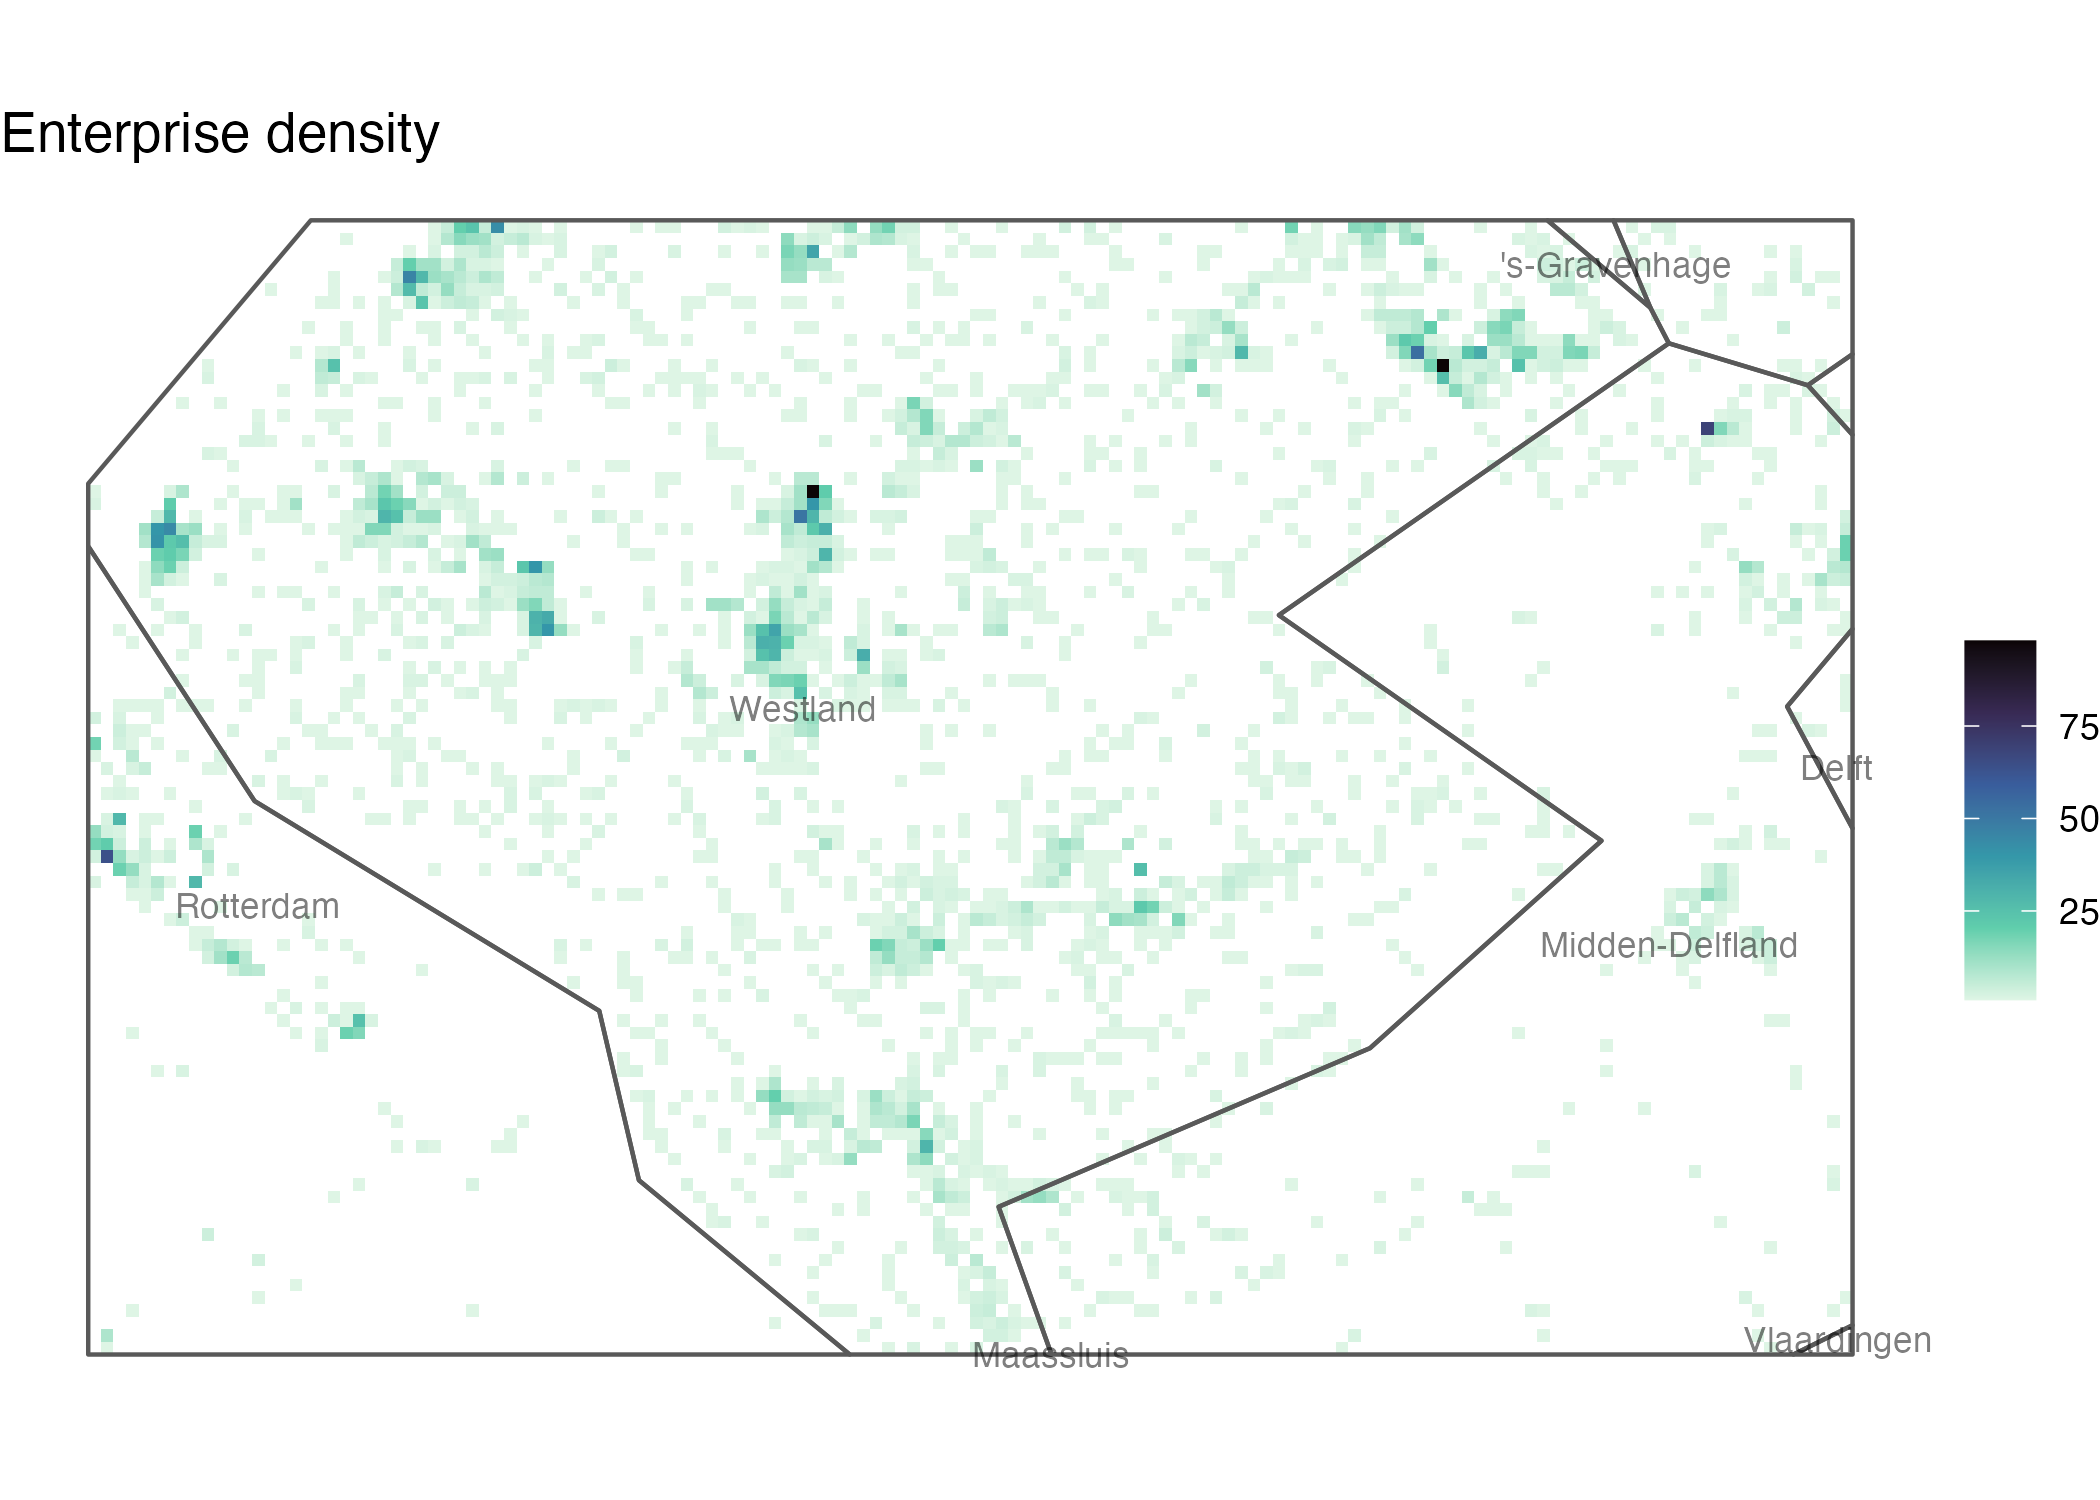
\includegraphics[width=.8\linewidth]{figures/Smoothing/enterprise_density.png} \\
    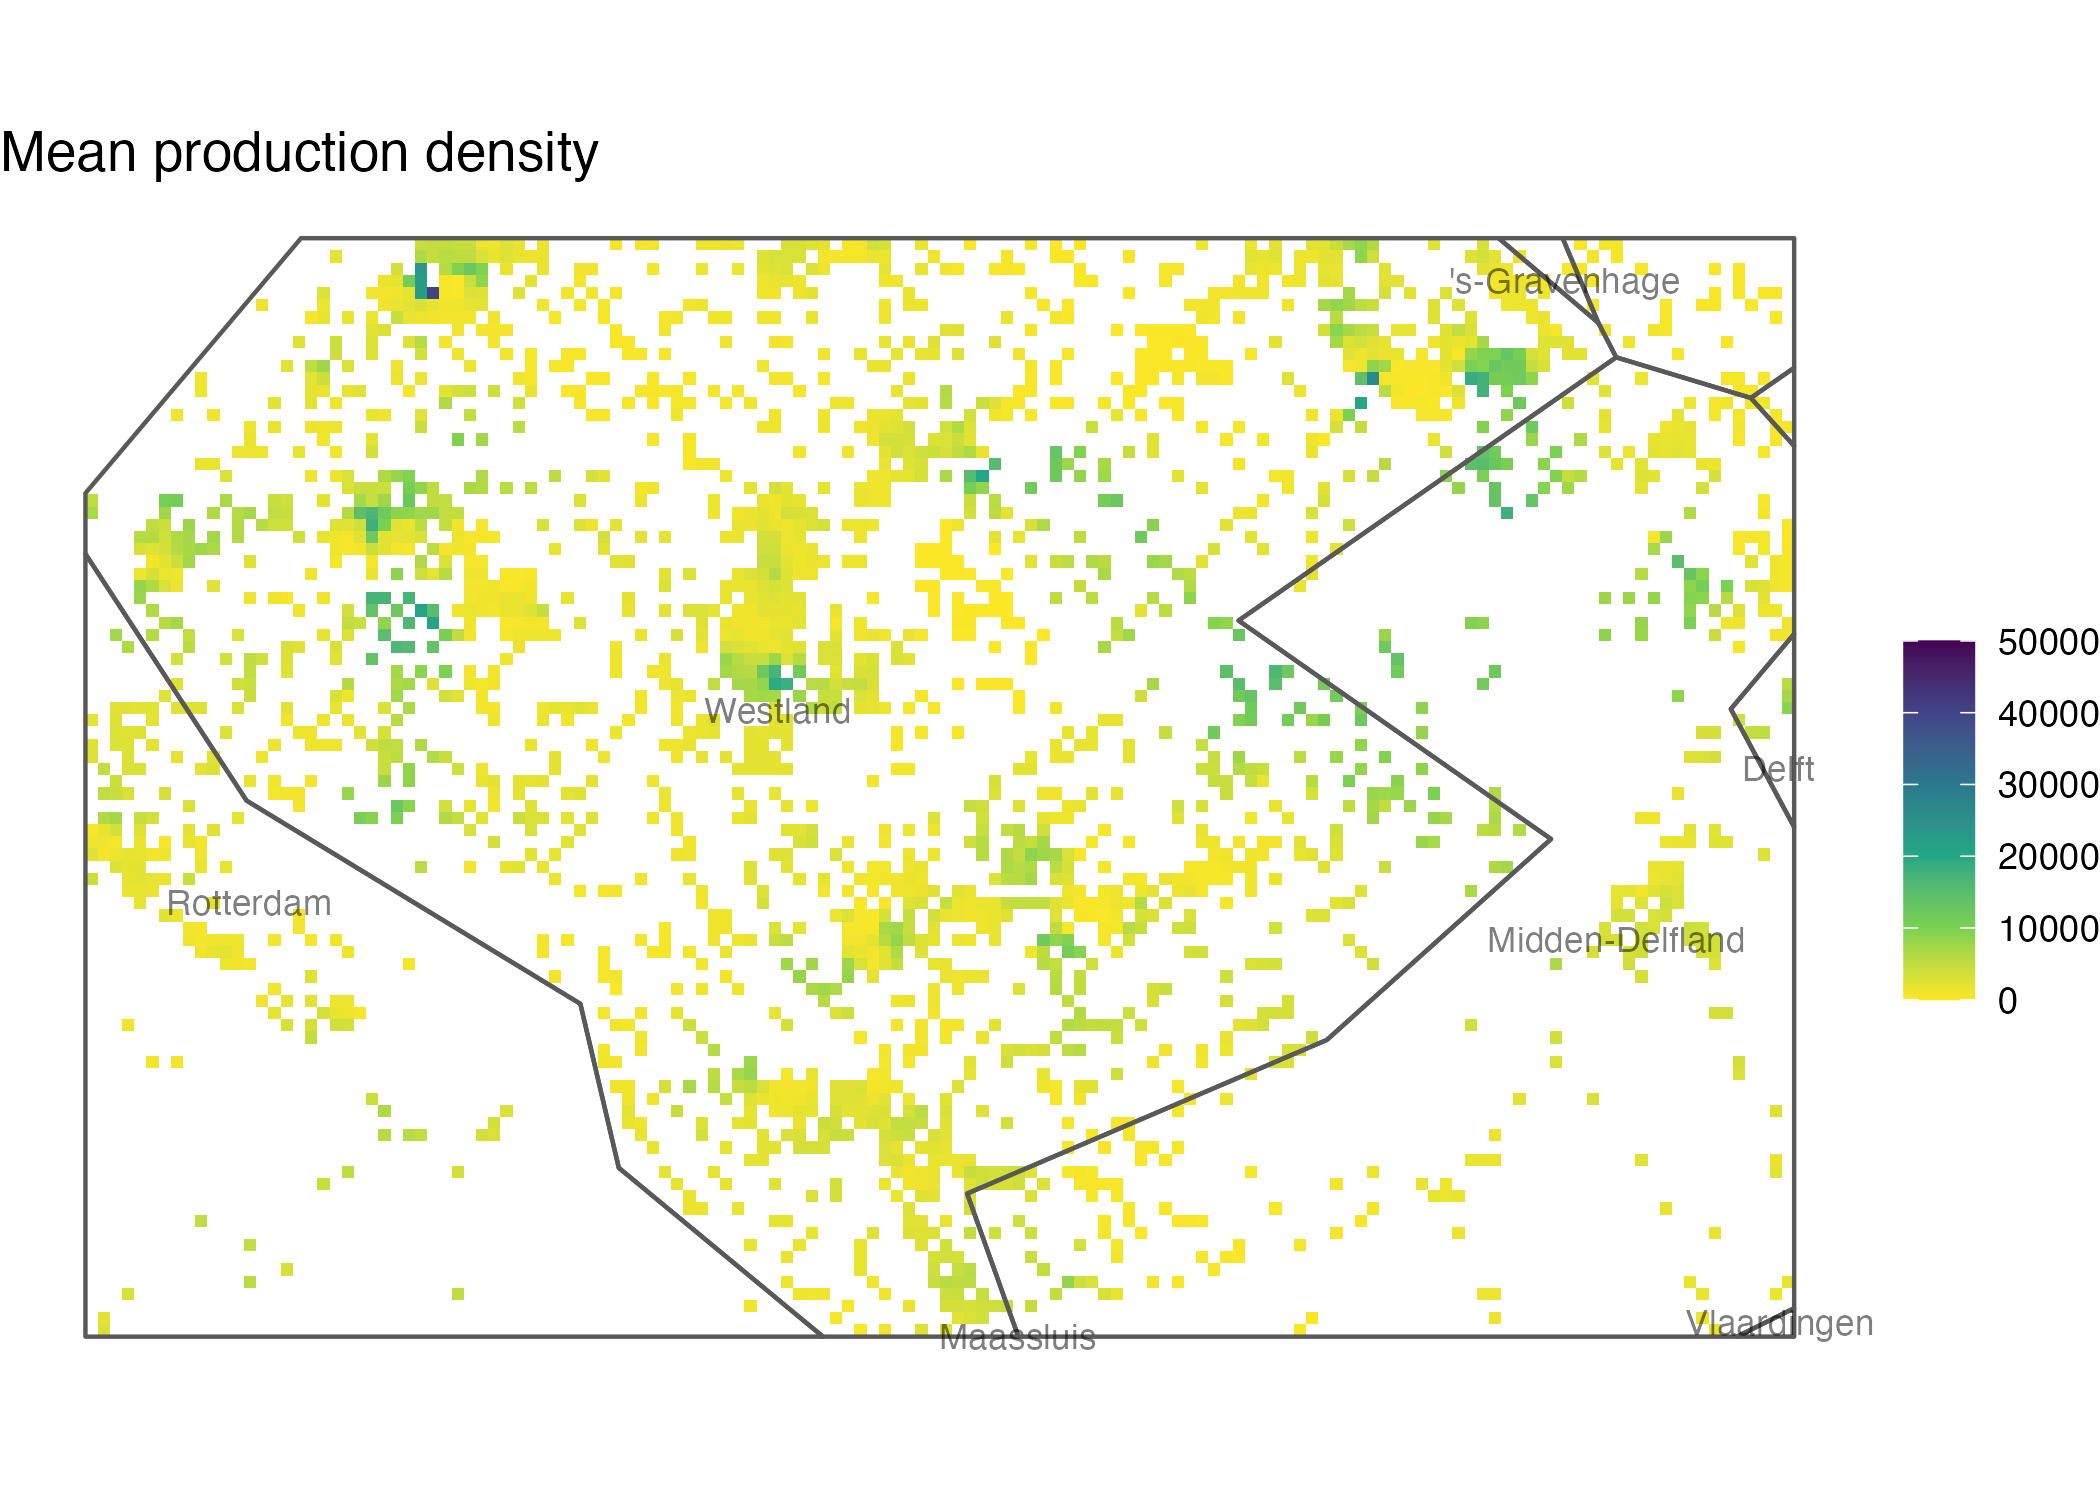
\includegraphics[width=.8\linewidth]{figures/Smoothing/mean_production_density.png}
    \caption{Density of enterprises (realistic) and their mean production (fictitious), created using \texttt{sdcSpatial} \citep{sdcSpatial_2022}}
    \label{fig:sm_density}
\end{figure}

Many geographical phenomena have
a skewed spatial distribution as figure \ref{fig:sm_density} exemplifies: enterprises and houses tend to cluster in 
geographical space. The enterprises are plotted in a 100m square grid, in which each grid cell contains the number of enterprises and the mean production within that grid cell. 

Common sense and figure \ref{fig:sm_sensitive} shows that most grid cells are unsafe for publication (in red), since most cells contain few enterprises: the cells of a 100m square grid are not expected to have high counts of enterprises.


\begin{figure}[H]
    \centering
    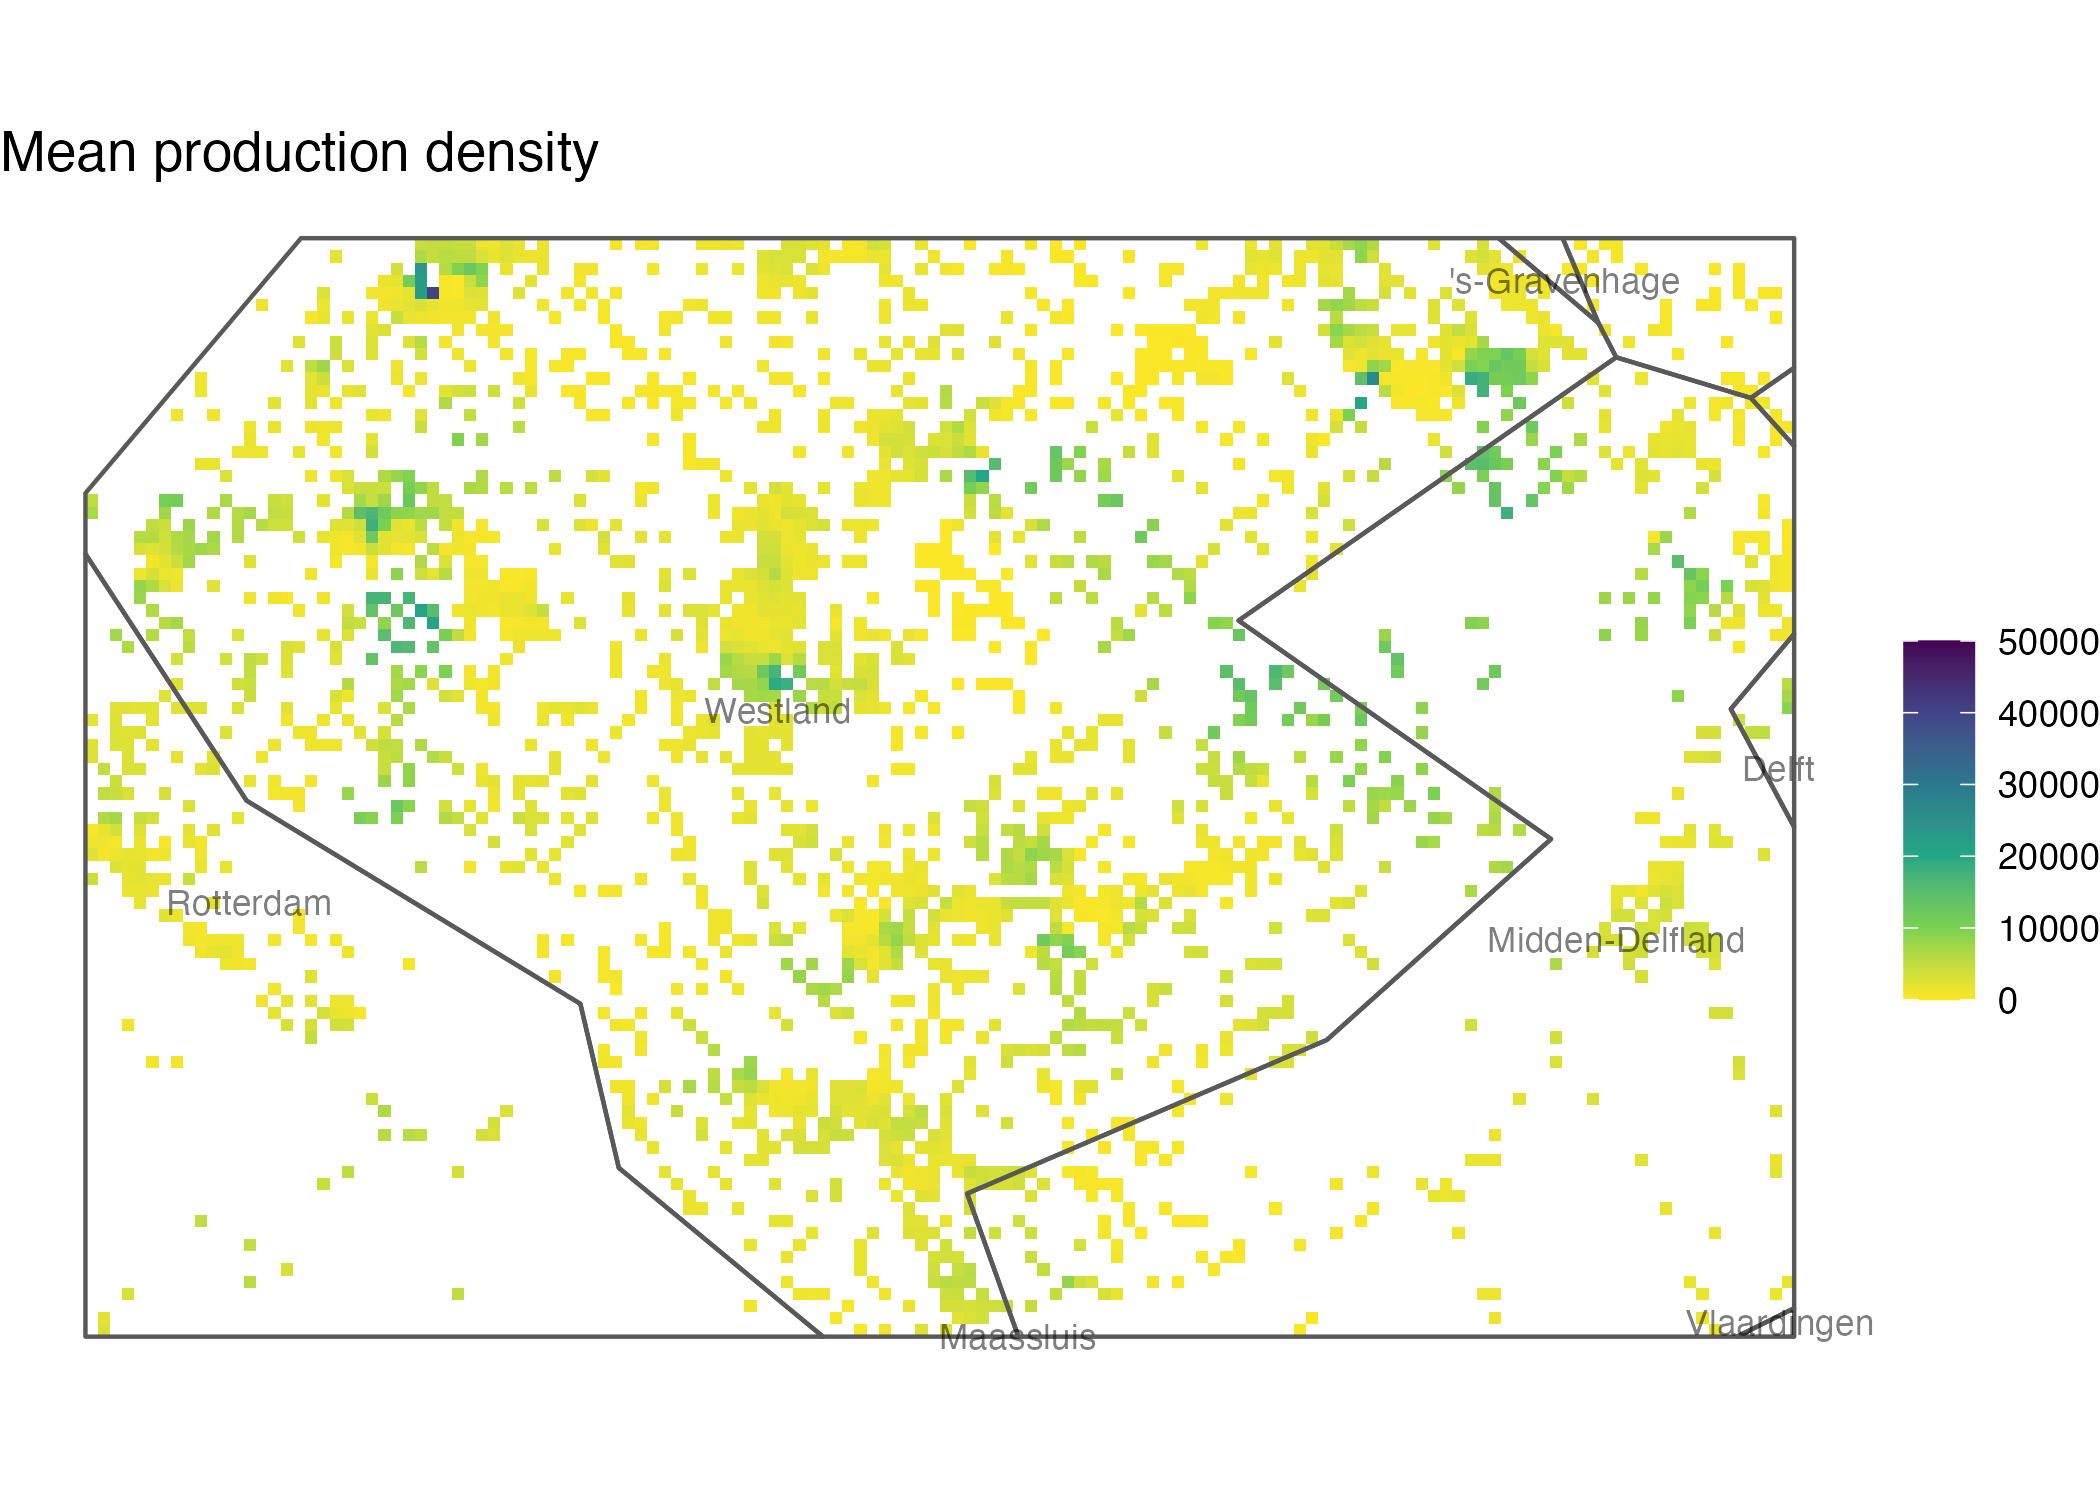
\includegraphics[width=.8\linewidth]{figures/Smoothing/mean_production_density.png} \\
    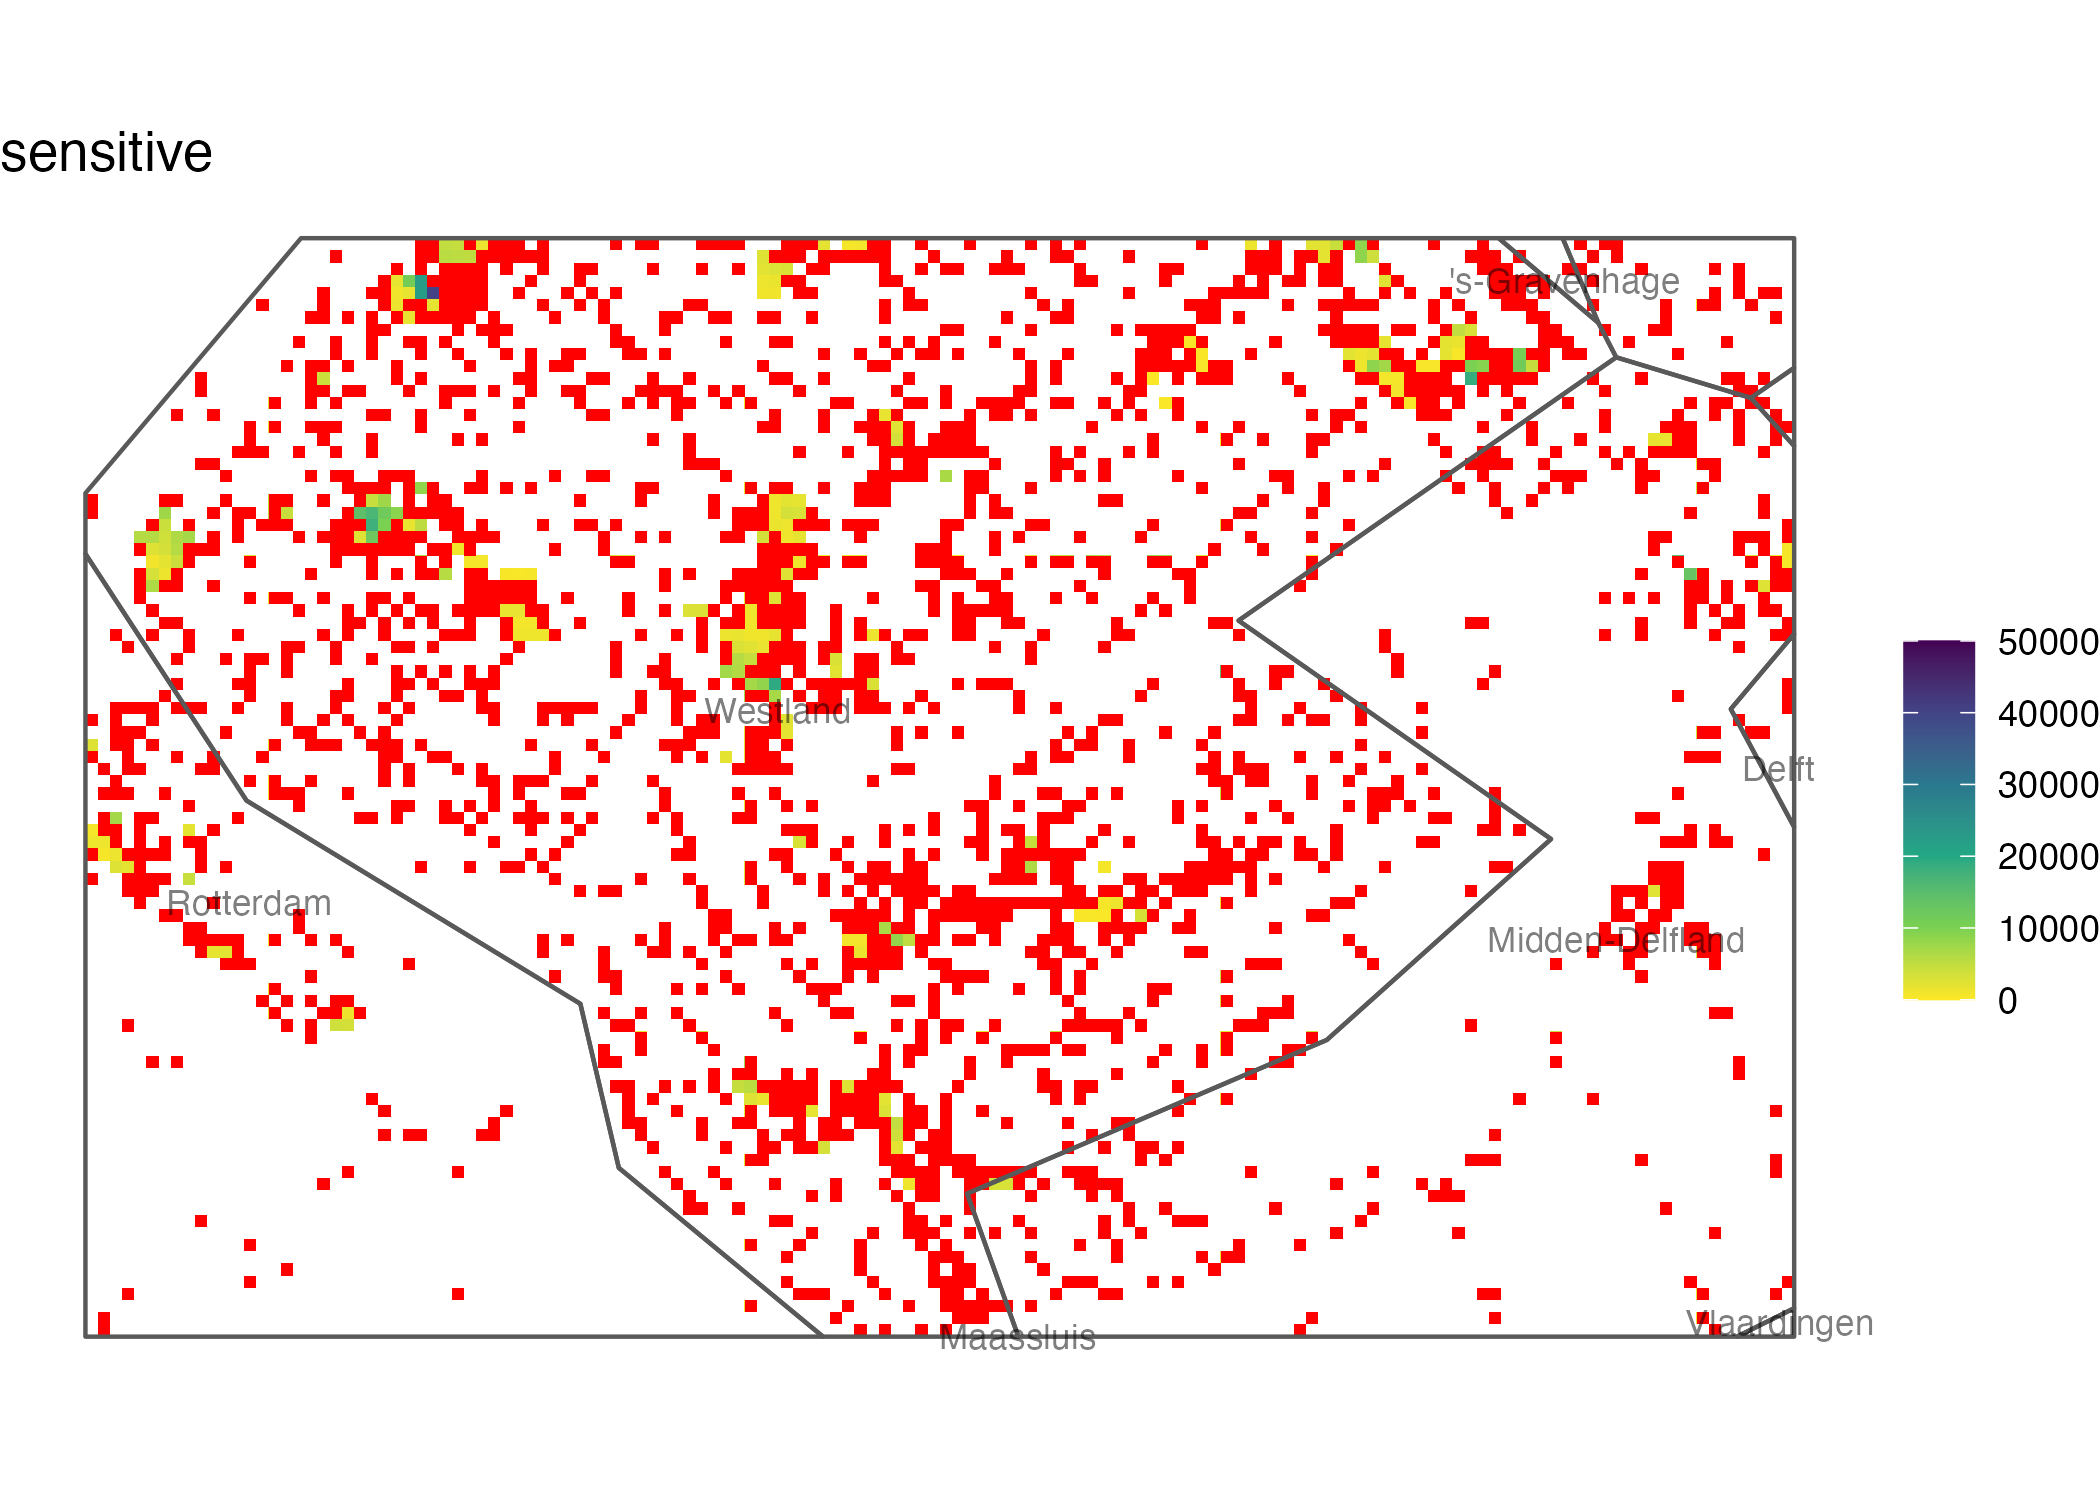
\includegraphics[width=.8\linewidth]{figures/Smoothing/sensitive.png}
    \caption{Mean production (left) and which grid cells are sensitive (right); most have too few enterprises to be safe.}
    \label{fig:sm_sensitive}
\end{figure}

\subsection{Spatial grid and resolution}

Equation (\ref{e:smooth}) is defined with $\vec{r}$ on $\mathbbm{R}^2$, 
but in practice a map is made discrete and published on a spatial grid
with a certain resolution. Furthermore, the computation of a spatial smoothing operation includes a spatial grid, e.g. it results in a dataset which has a fixed spatial resolution.

It is useful to define the risk function using a grid cell in the spatial grid. E.g. $k$-anonymity can easily be defined per grid cell as well as
$(n,k)$ dominance. 

A simple solution to reduce the disclosure risk is by coarsening the grid as 
is shown in figure \ref{fig:sm_resolution_dep}: plotting the data 
on increasingly coarser grids, i.e. with an increasing minimal resolution.

\begin{figure}[H]
    \centering
    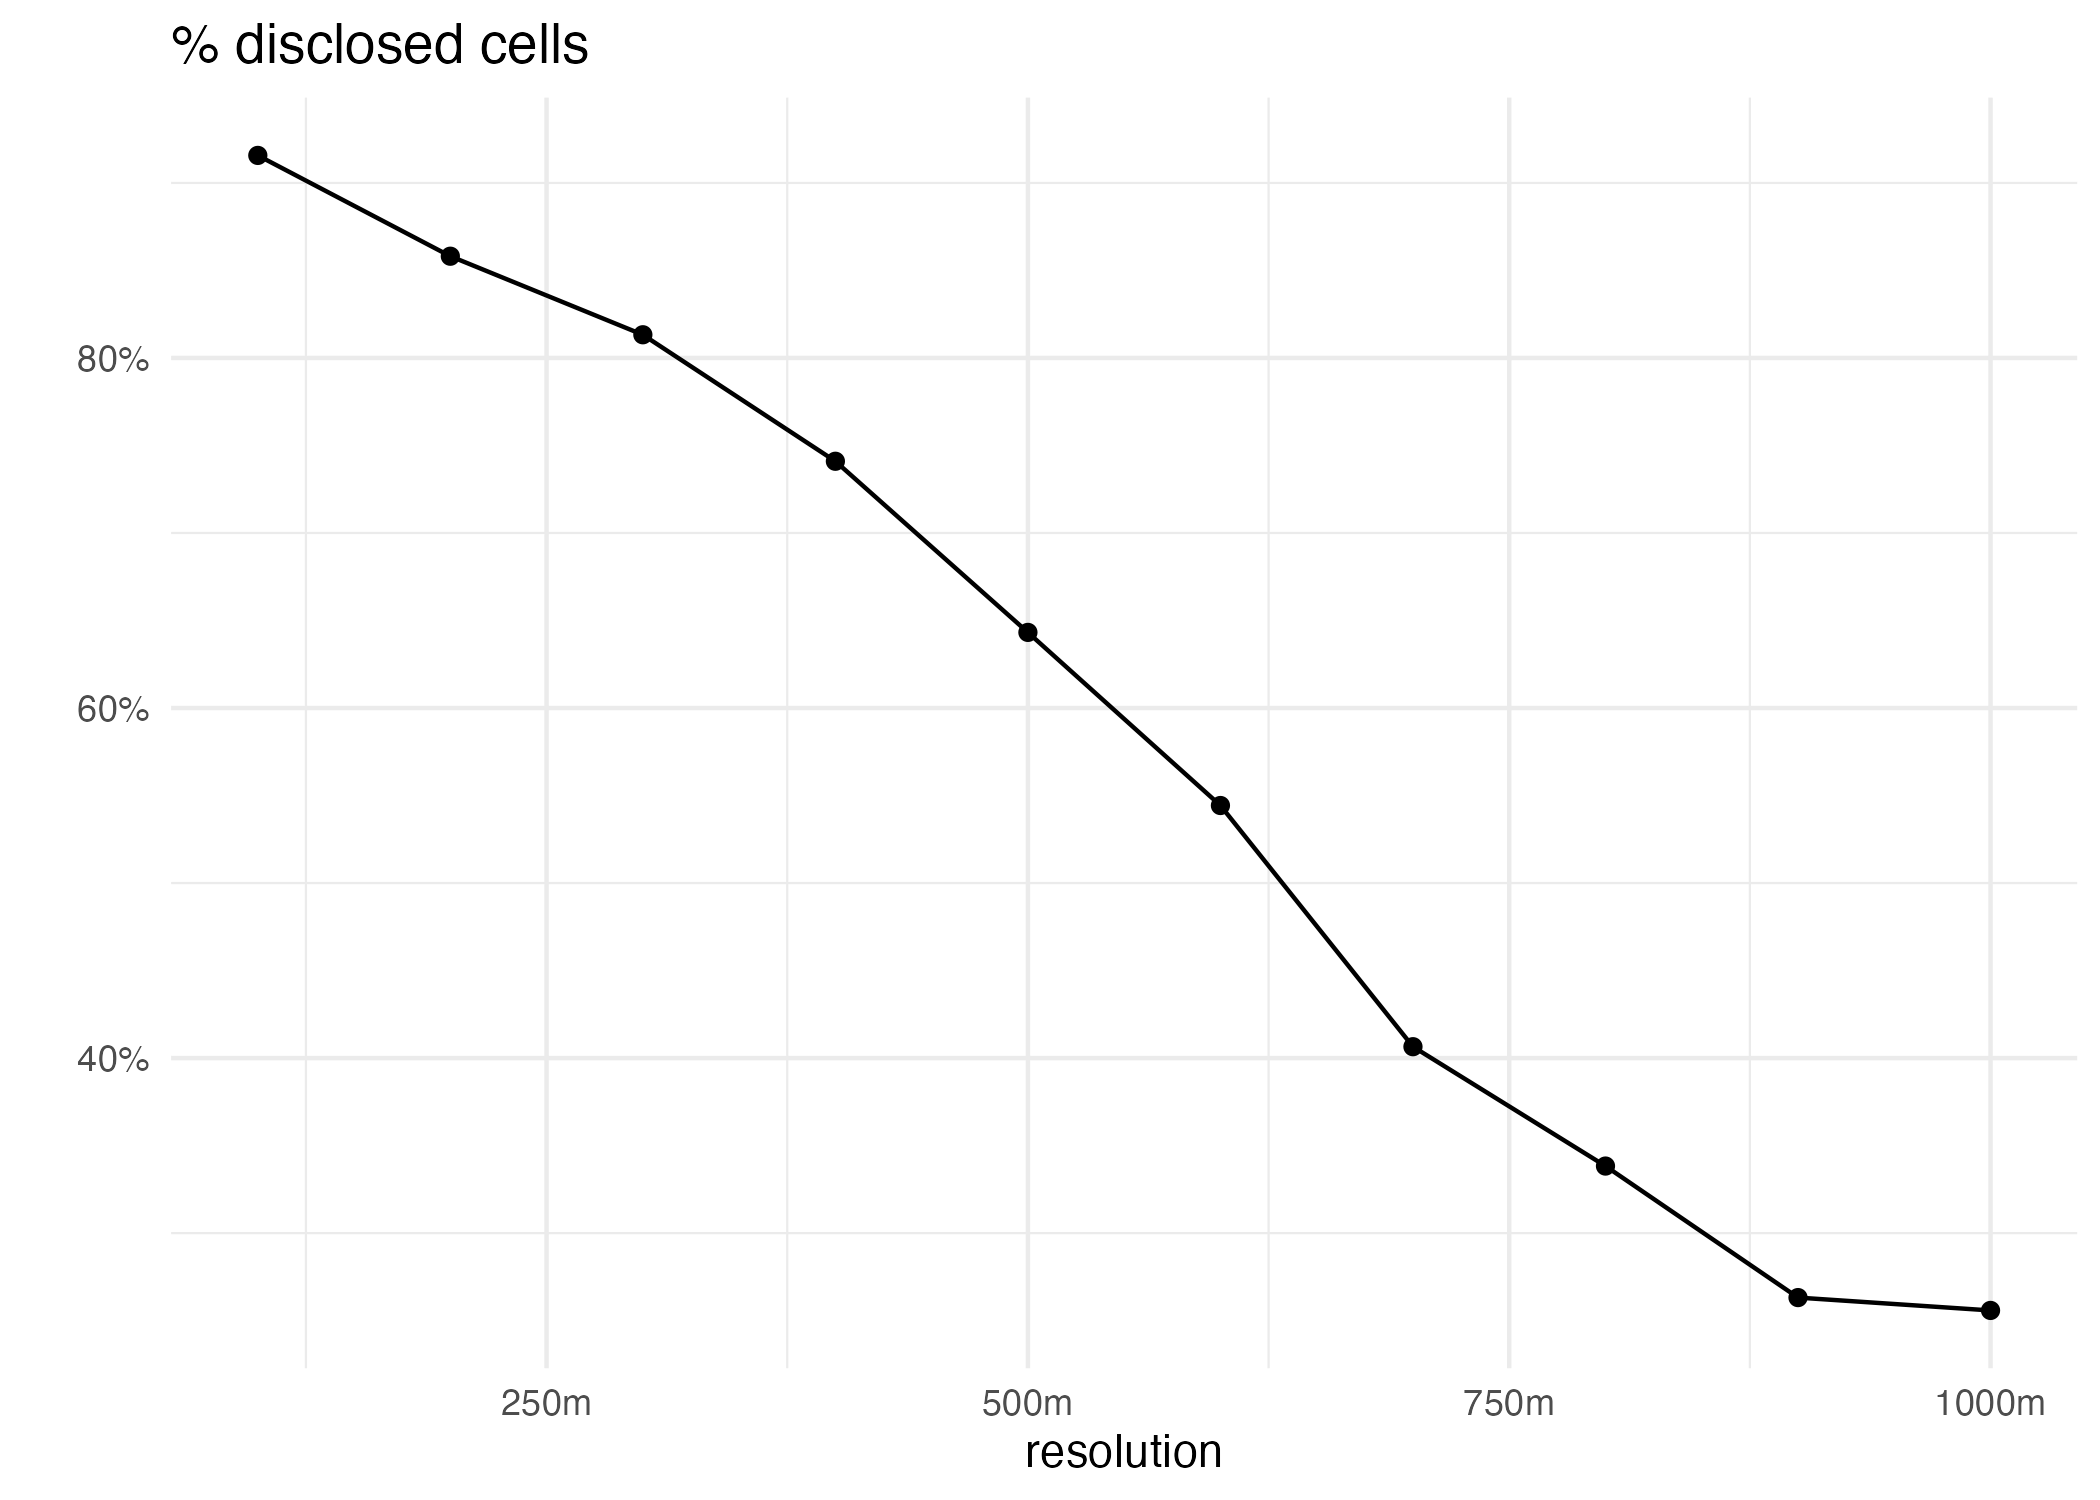
\includegraphics[width=.8\linewidth]{figures/Smoothing/sensitive_res.png}
    \caption{Disclosure risk for the dataset with increasing minimal resolution.}
    \label{fig:sm_resolution_dep}
\end{figure}

The risk-utility trade off can be seen in figure \ref{fig:sm_resolution}:
with increasing resolution, the resulting map becomes more blocky.

\begin{figure}[H]
    \centering
    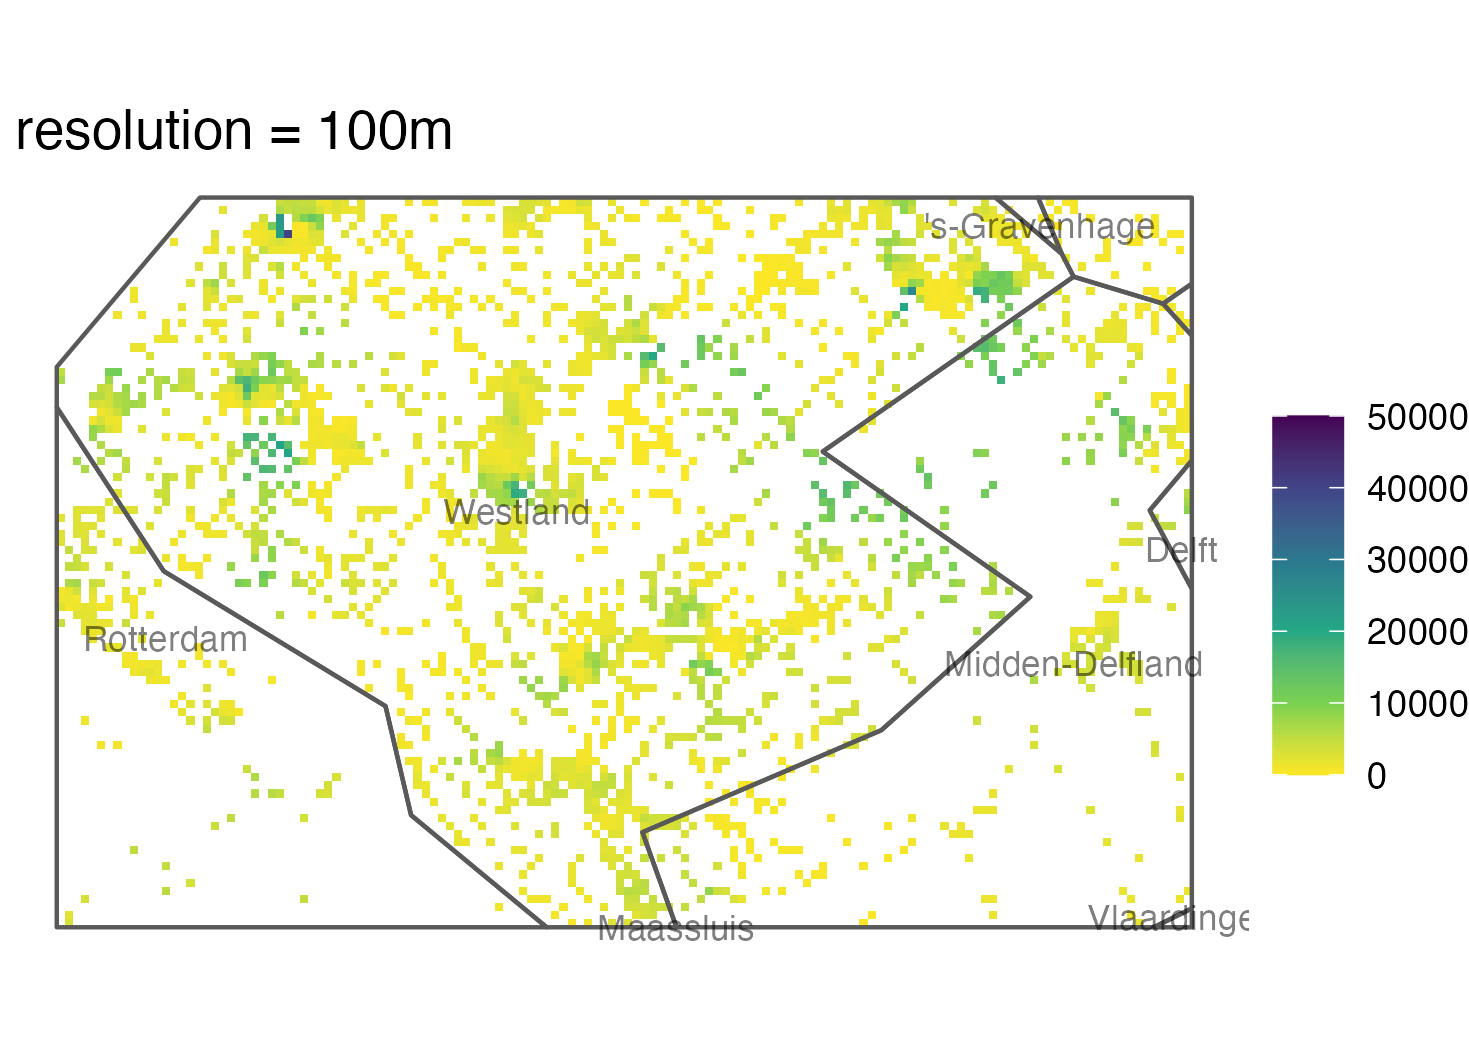
\includegraphics[width=.49\linewidth]{figures/Smoothing/res_100.png}
    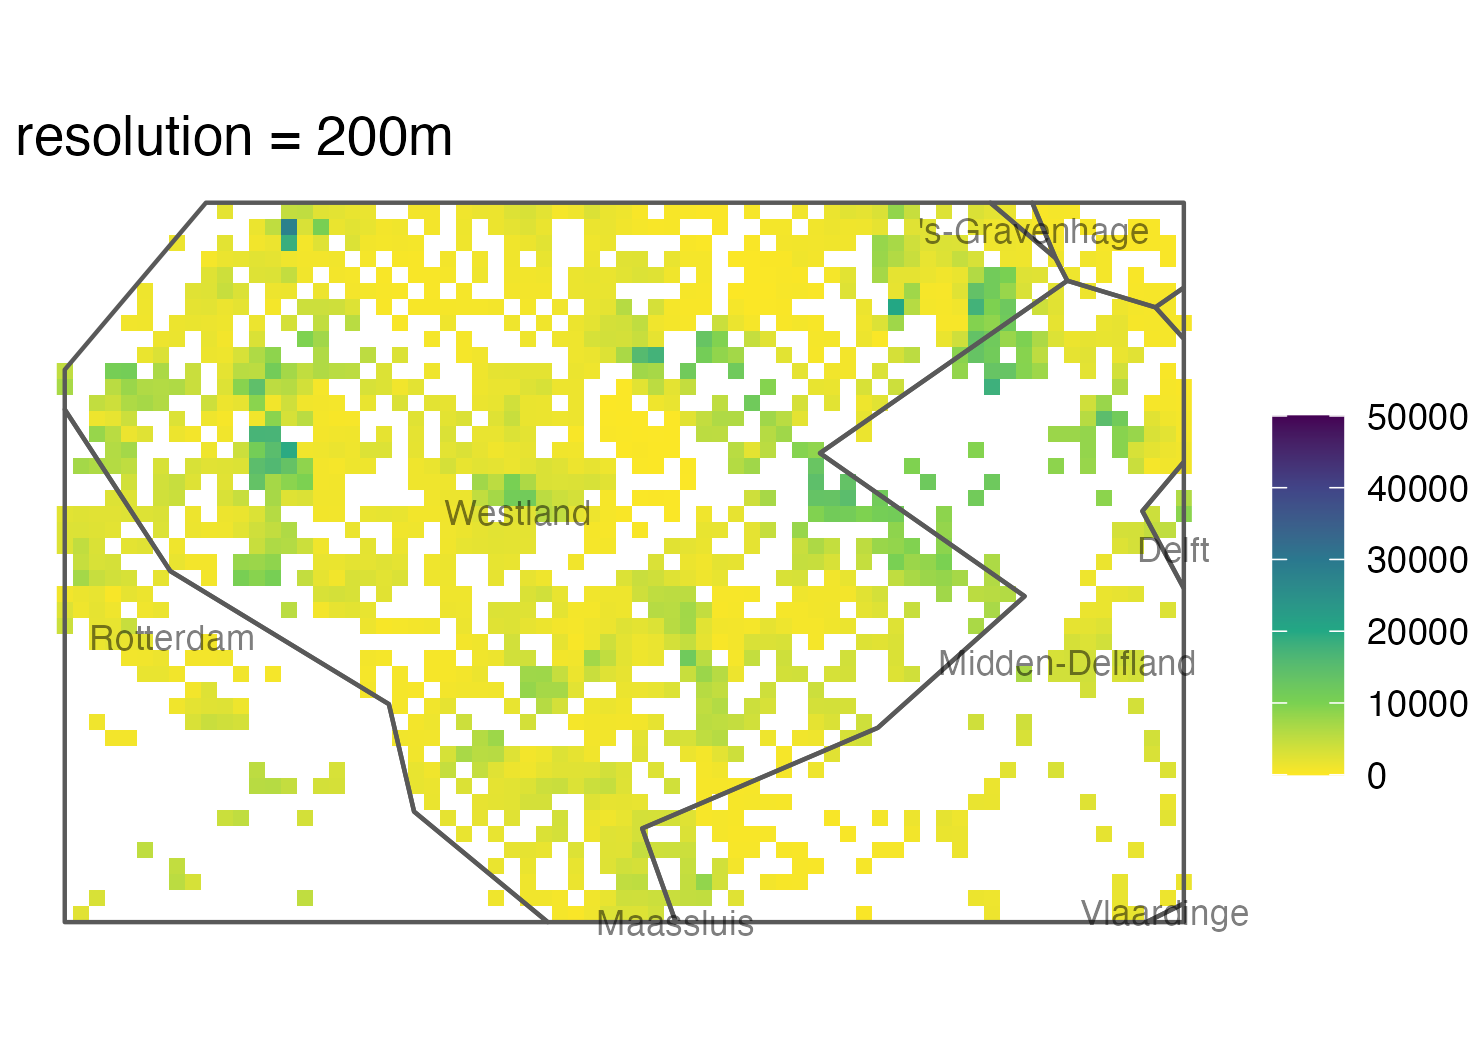
\includegraphics[width=.49\linewidth]{figures/Smoothing/res_200.png}\\
    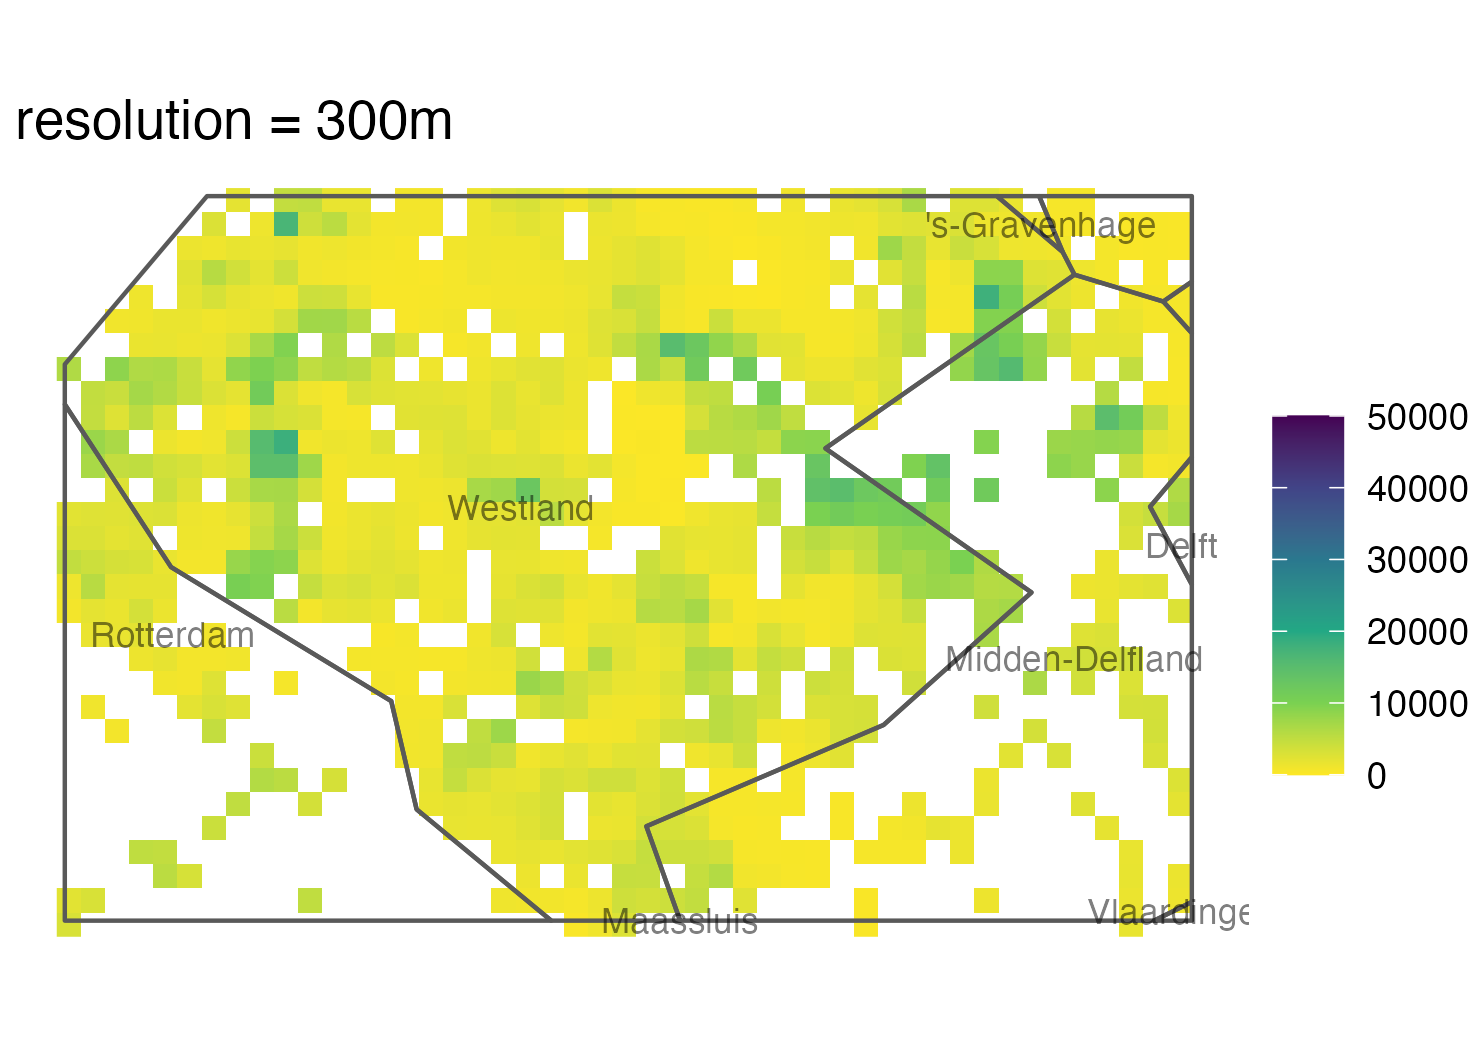
\includegraphics[width=.49\linewidth]{figures/Smoothing/res_300.png}
    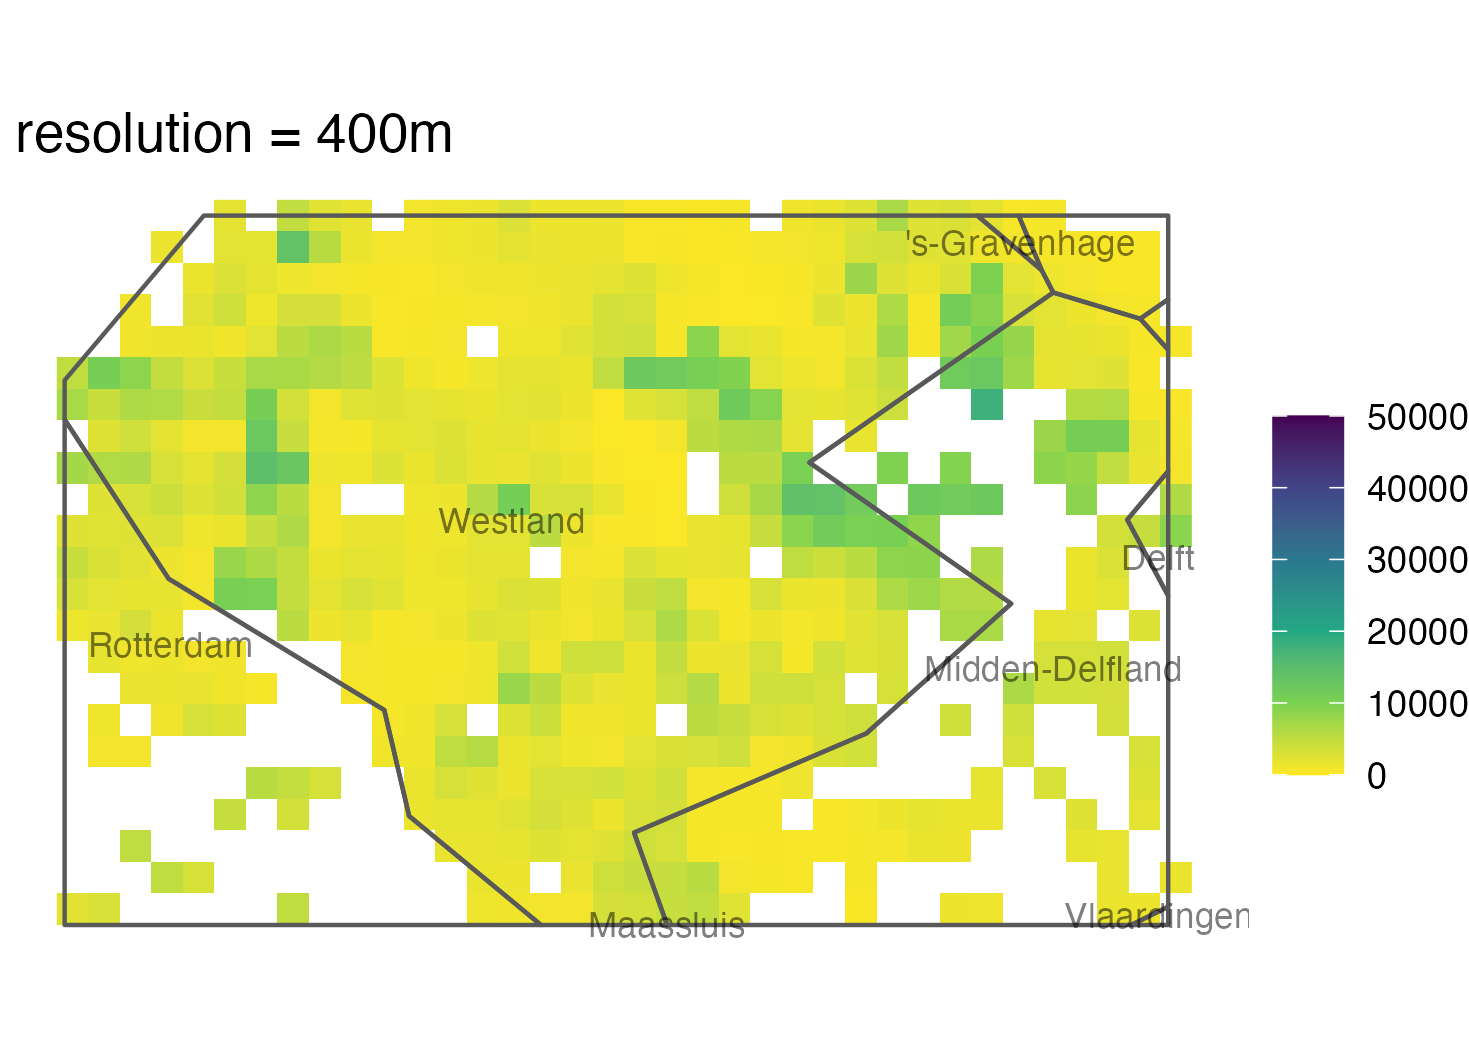
\includegraphics[width=.49\linewidth]{figures/Smoothing/res_400.png}\\
    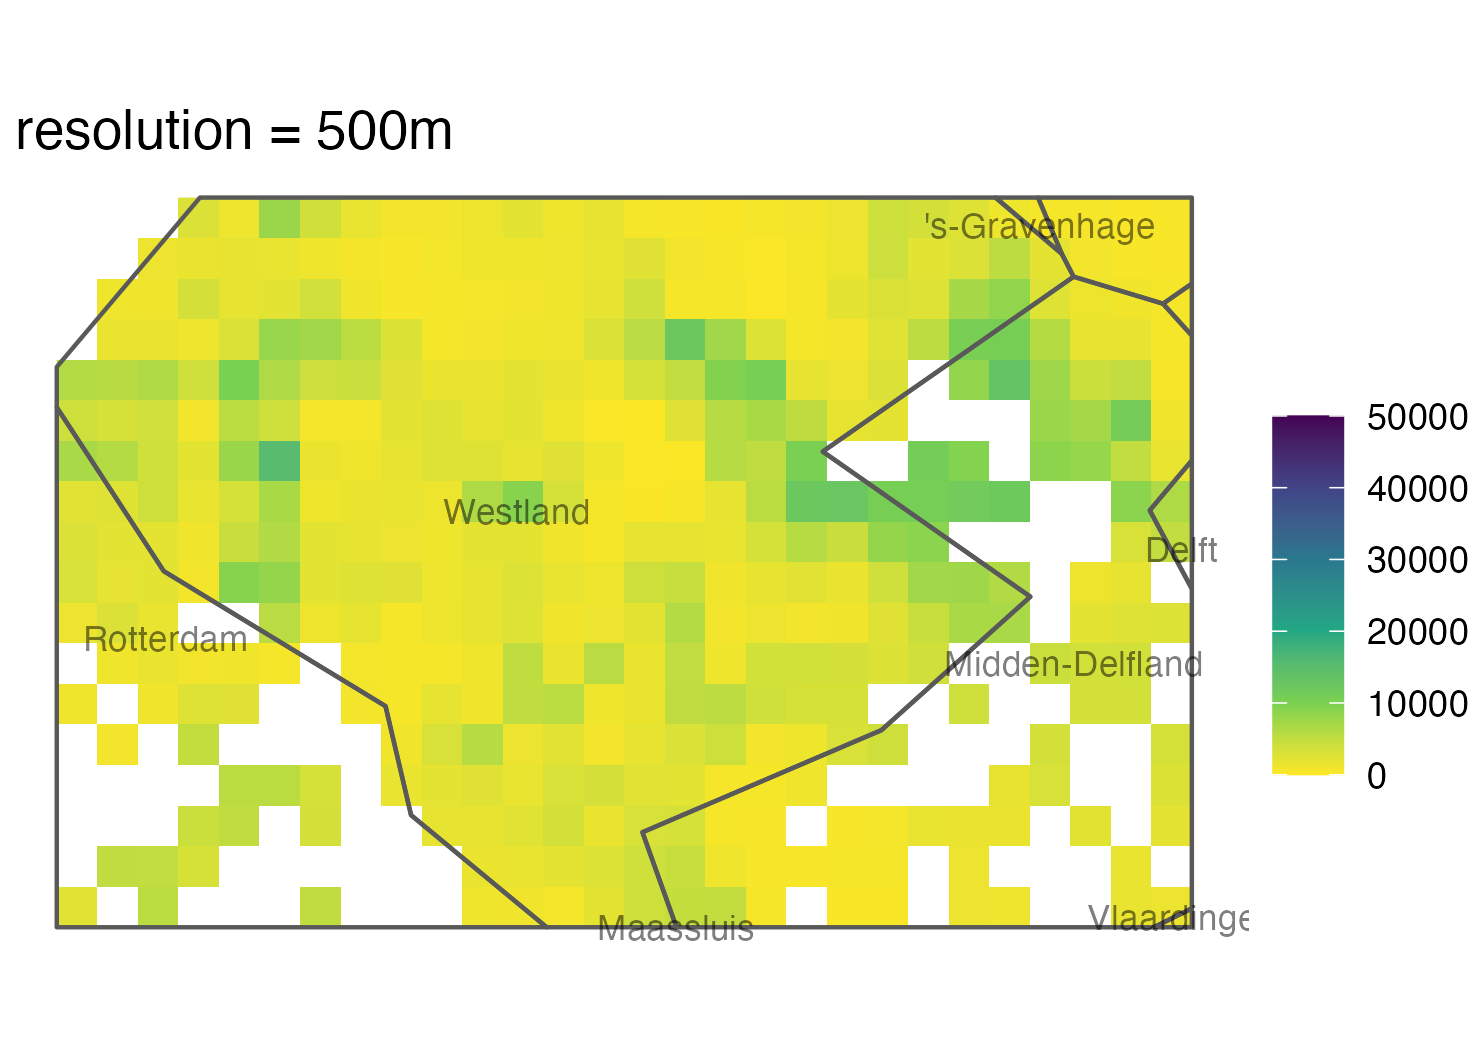
\includegraphics[width=.49\linewidth]{figures/Smoothing/res_500.png}
    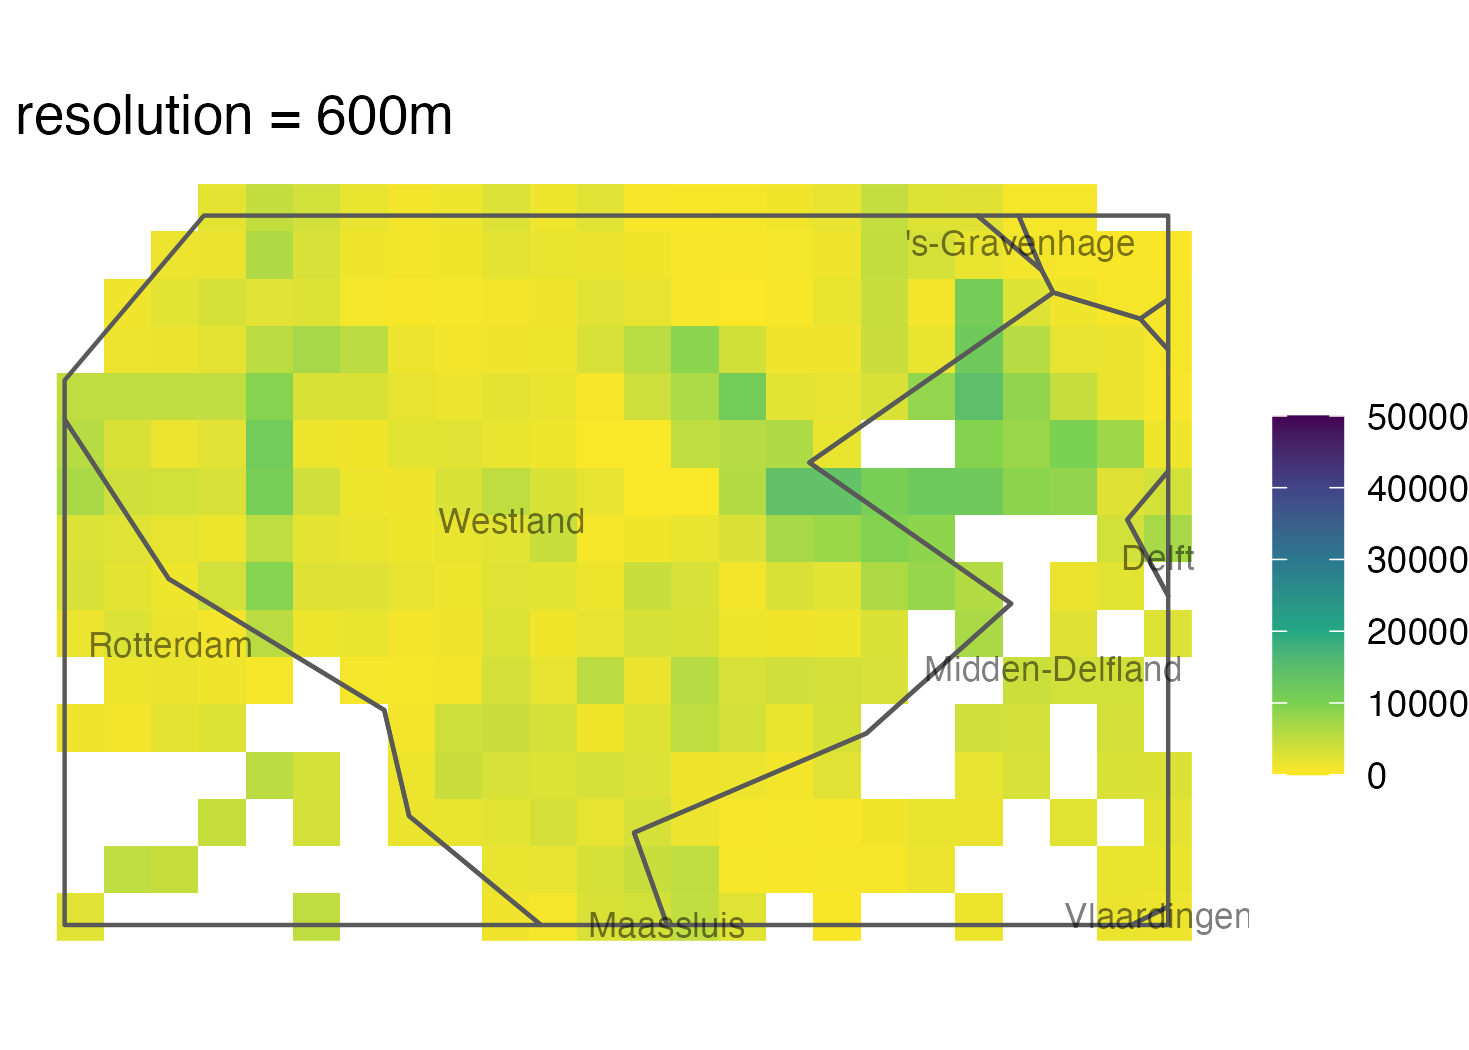
\includegraphics[width=.49\linewidth]{figures/Smoothing/res_600.png}\\
    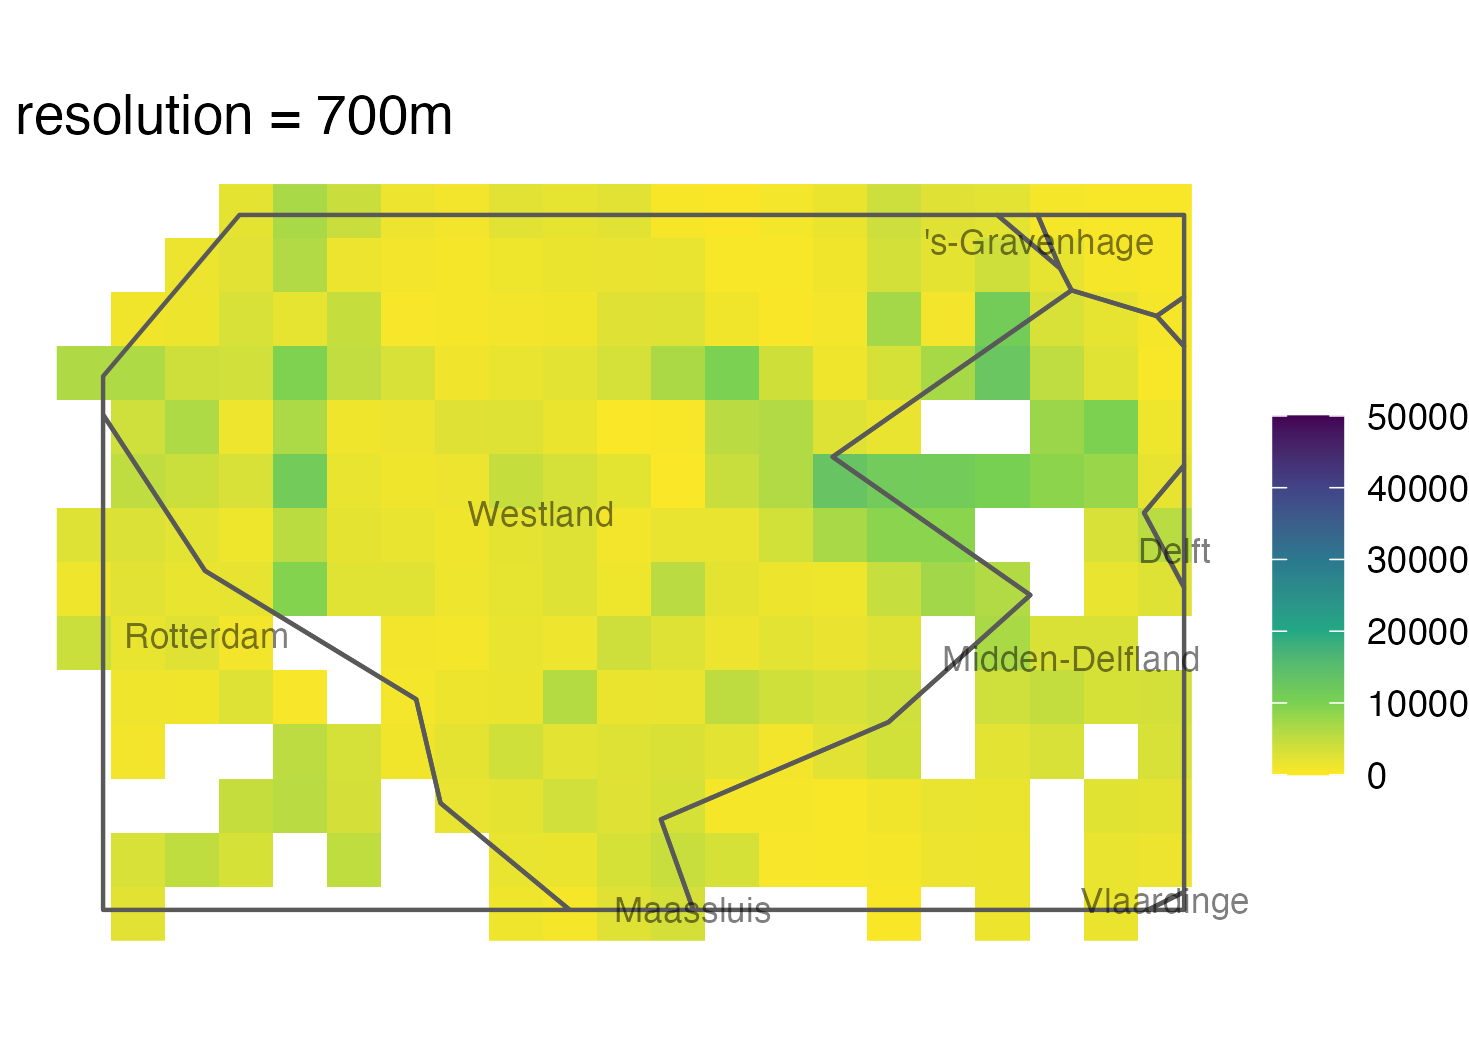
\includegraphics[width=.49\linewidth]{figures/Smoothing/res_700.png}
    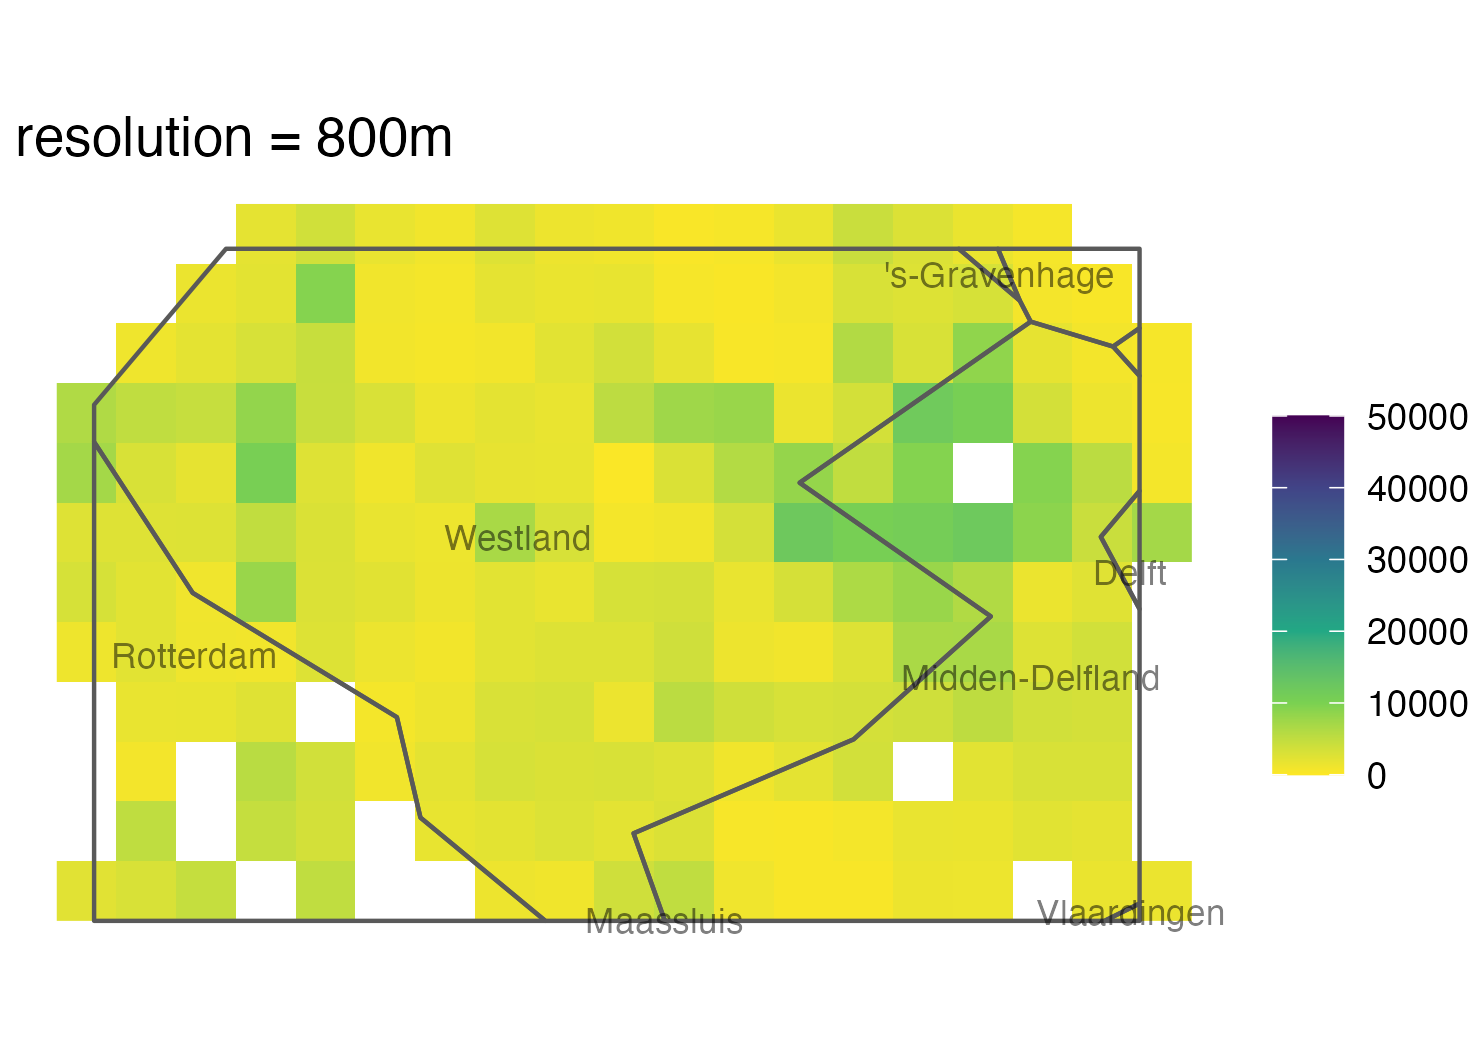
\includegraphics[width=.49\linewidth]{figures/Smoothing/res_800.png}\\
    \caption{Coarsening the grid by increasing the resolution (100-800m).}
    \label{fig:sm_resolution}
\end{figure}

Improving the utility of the map can be done by borrowing or blending values from 
neighboring cells: by smoothing using a Gaussian kernel smoother. 

\subsection{Risk and utility for band widths}

An other important parameter for kernel smoothing is the choice of the band width.
Increasing the band width reduces the number of unsafe locations and cells as
can be seen in figure \ref{fig:sm_sensitive_bw} where kernel smoothing is 
applied to the synthetic dataset. As sensitivity score, the $k$-anonymity with $k = 10$ is taken. When applying a smoothing operation on a spatial grid, the $k$-anonymity risk boundary is also smoothed.

\begin{figure}[H]
    \centering
    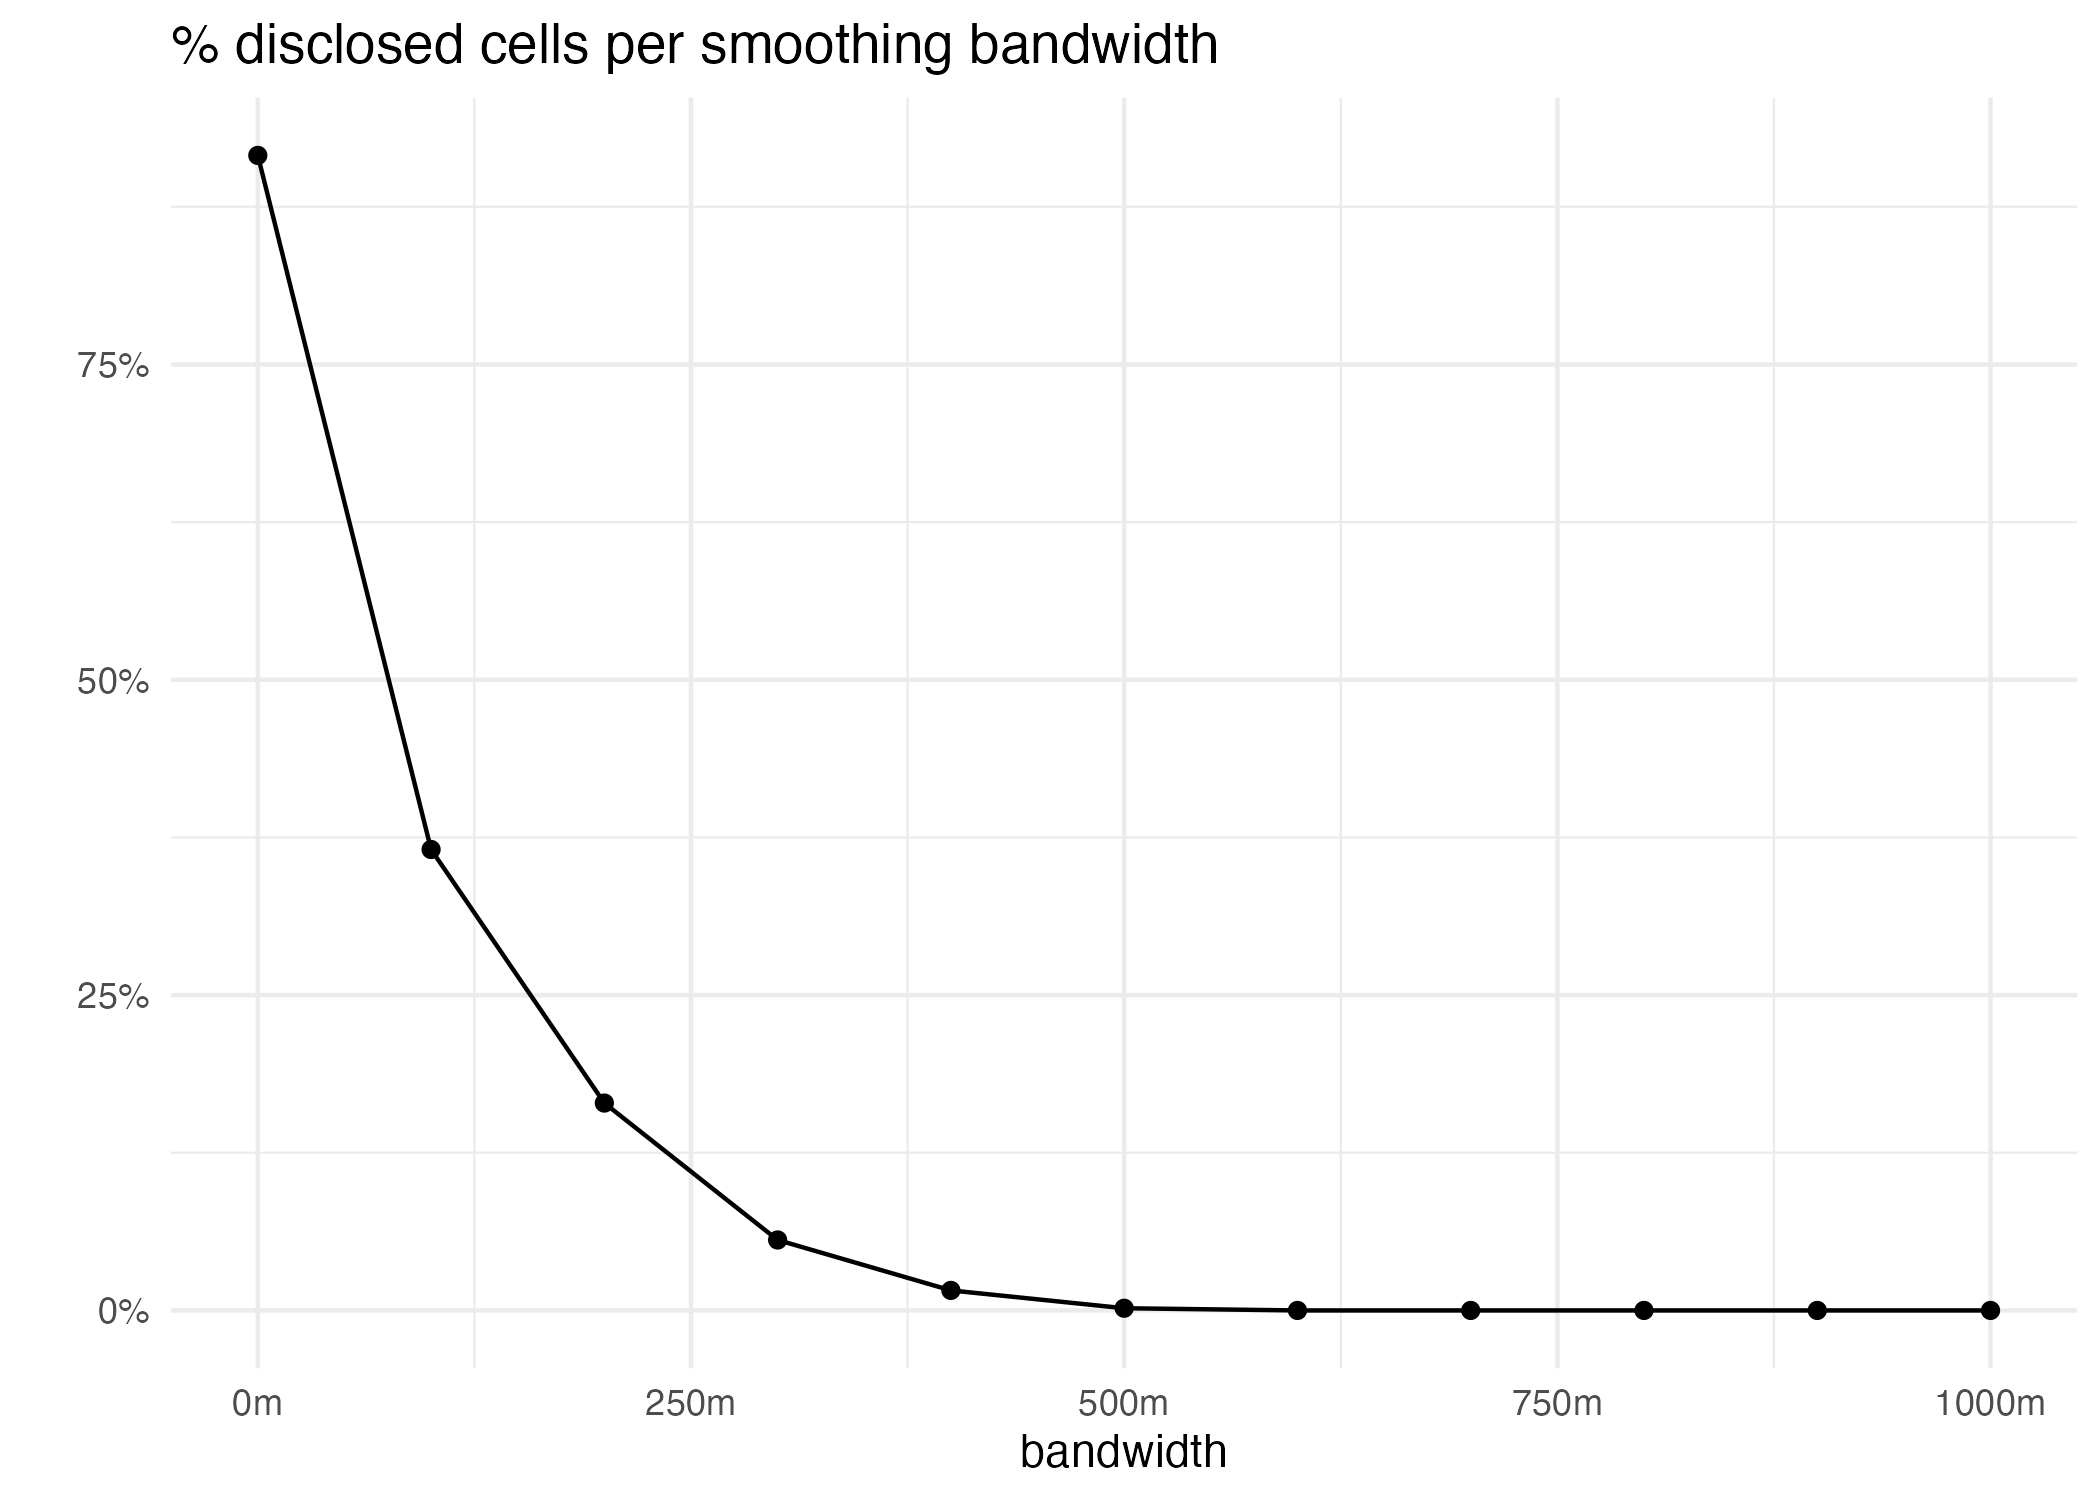
\includegraphics[width=.8\linewidth]{figures/Smoothing/sensitive_dep.png} 
    \caption{Unsafe locations as a function of the band width of the kernel density smoother.}
    \label{fig:sm_sensitive_bw}
\end{figure}

The trade off between risk and utility can be seen in figure~\ref{fig:sm_bandwidth}, which shows that for larger band widths, the spatial pattern is smoothed away. Interestingly enough smoothing with small band widths seems to improve visual utility, by improving spatial pattern. For the location utility measures however, it performs worse than 
other protection measures.

\begin{figure}[H]
    \centering
    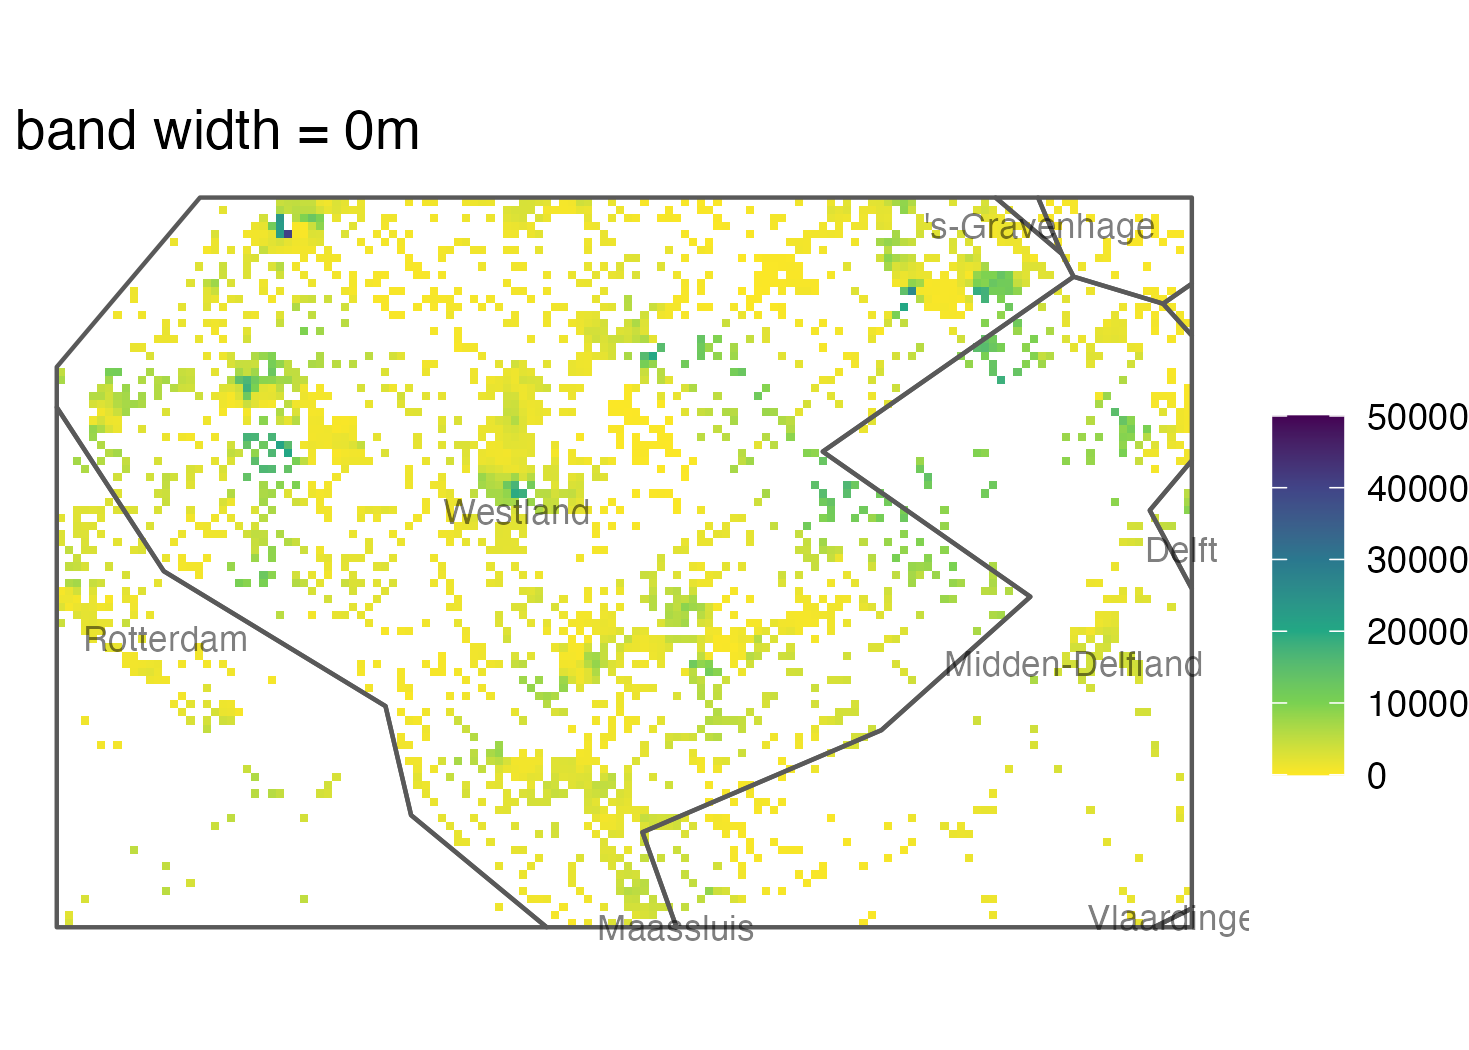
\includegraphics[width=.49\linewidth]{figures/Smoothing/fixed_smooth_0.png}
    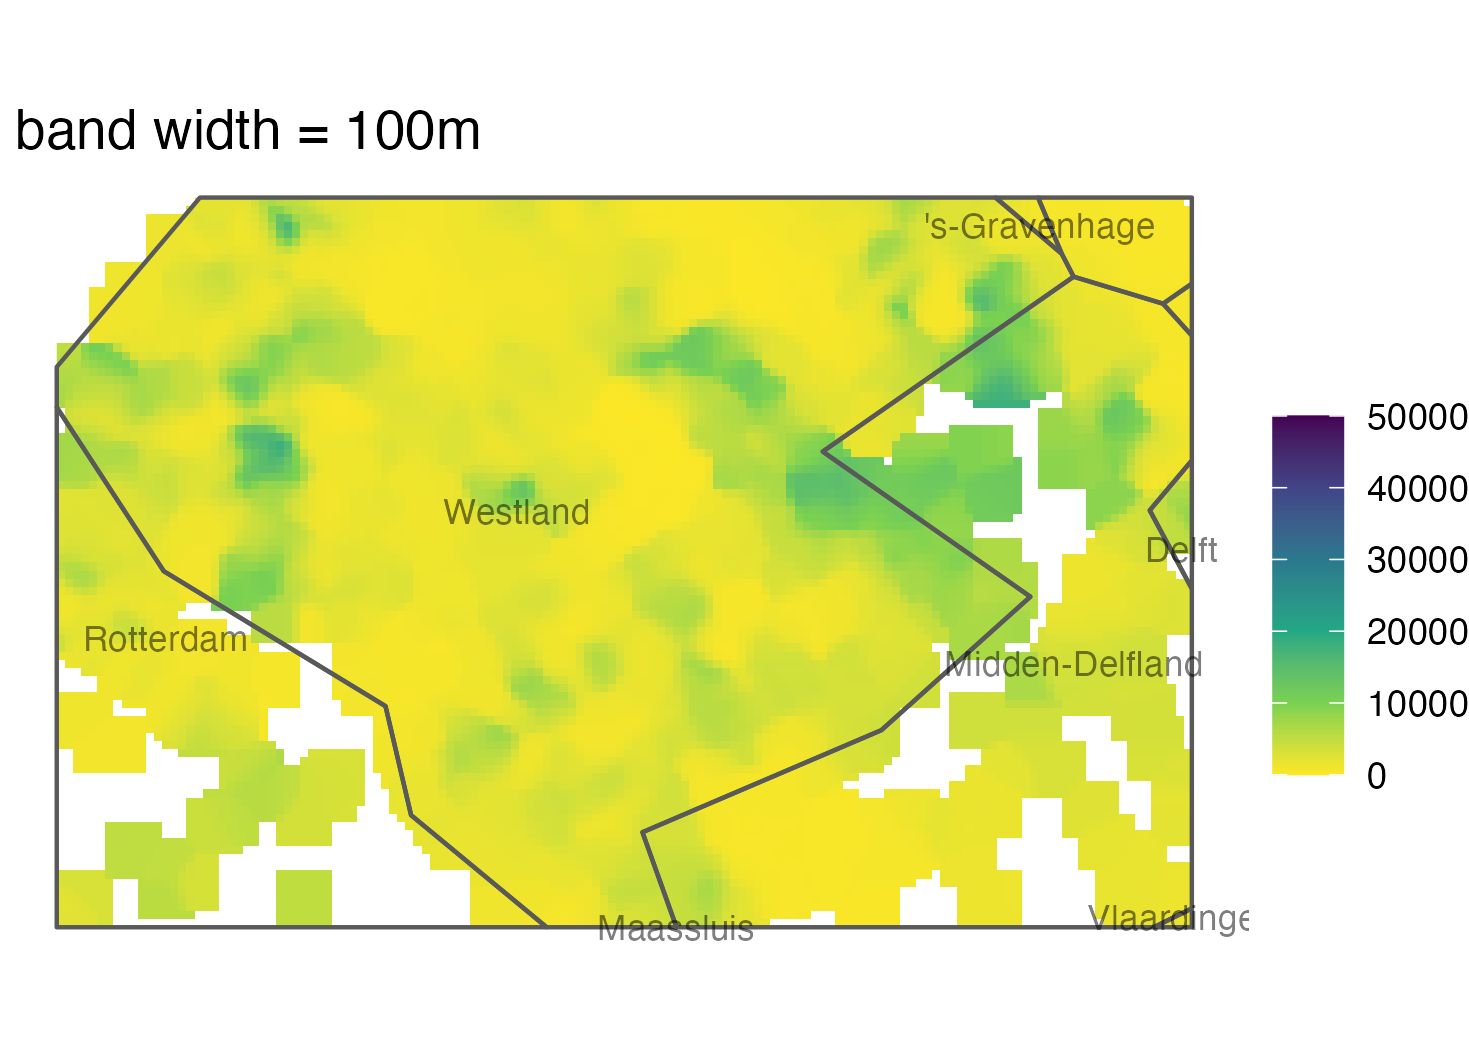
\includegraphics[width=.49\linewidth]{figures/Smoothing/fixed_smooth_100.png}\\
    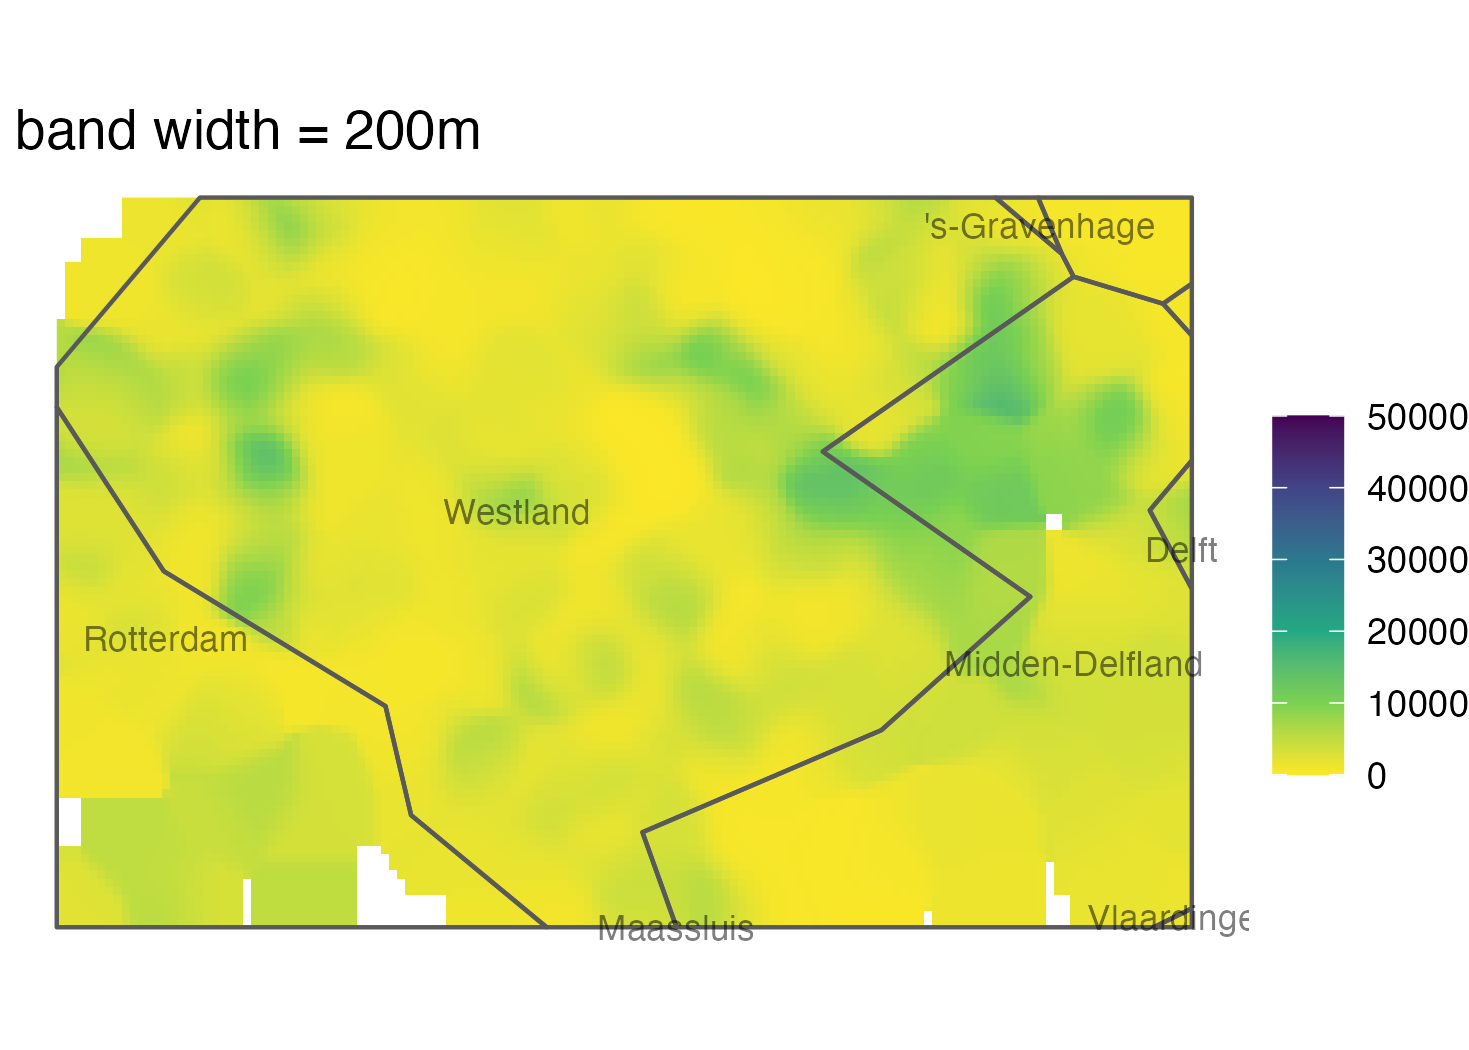
\includegraphics[width=.49\linewidth]{figures/Smoothing/fixed_smooth_200.png} 
    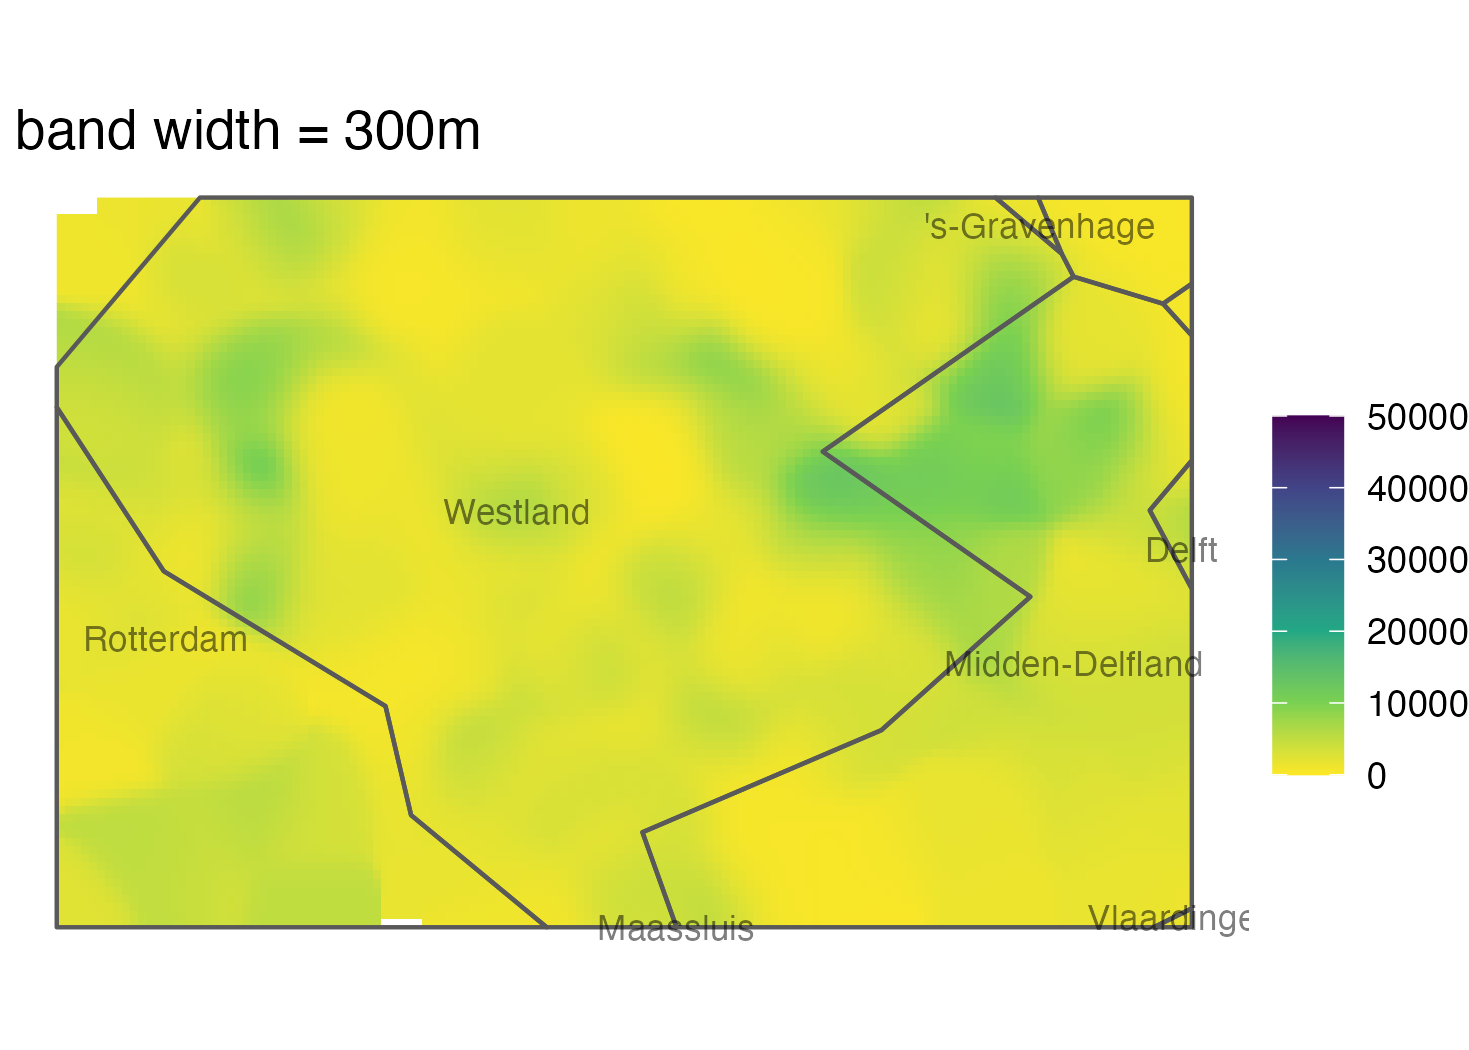
\includegraphics[width=.49\linewidth]{figures/Smoothing/fixed_smooth_300.png} \\
    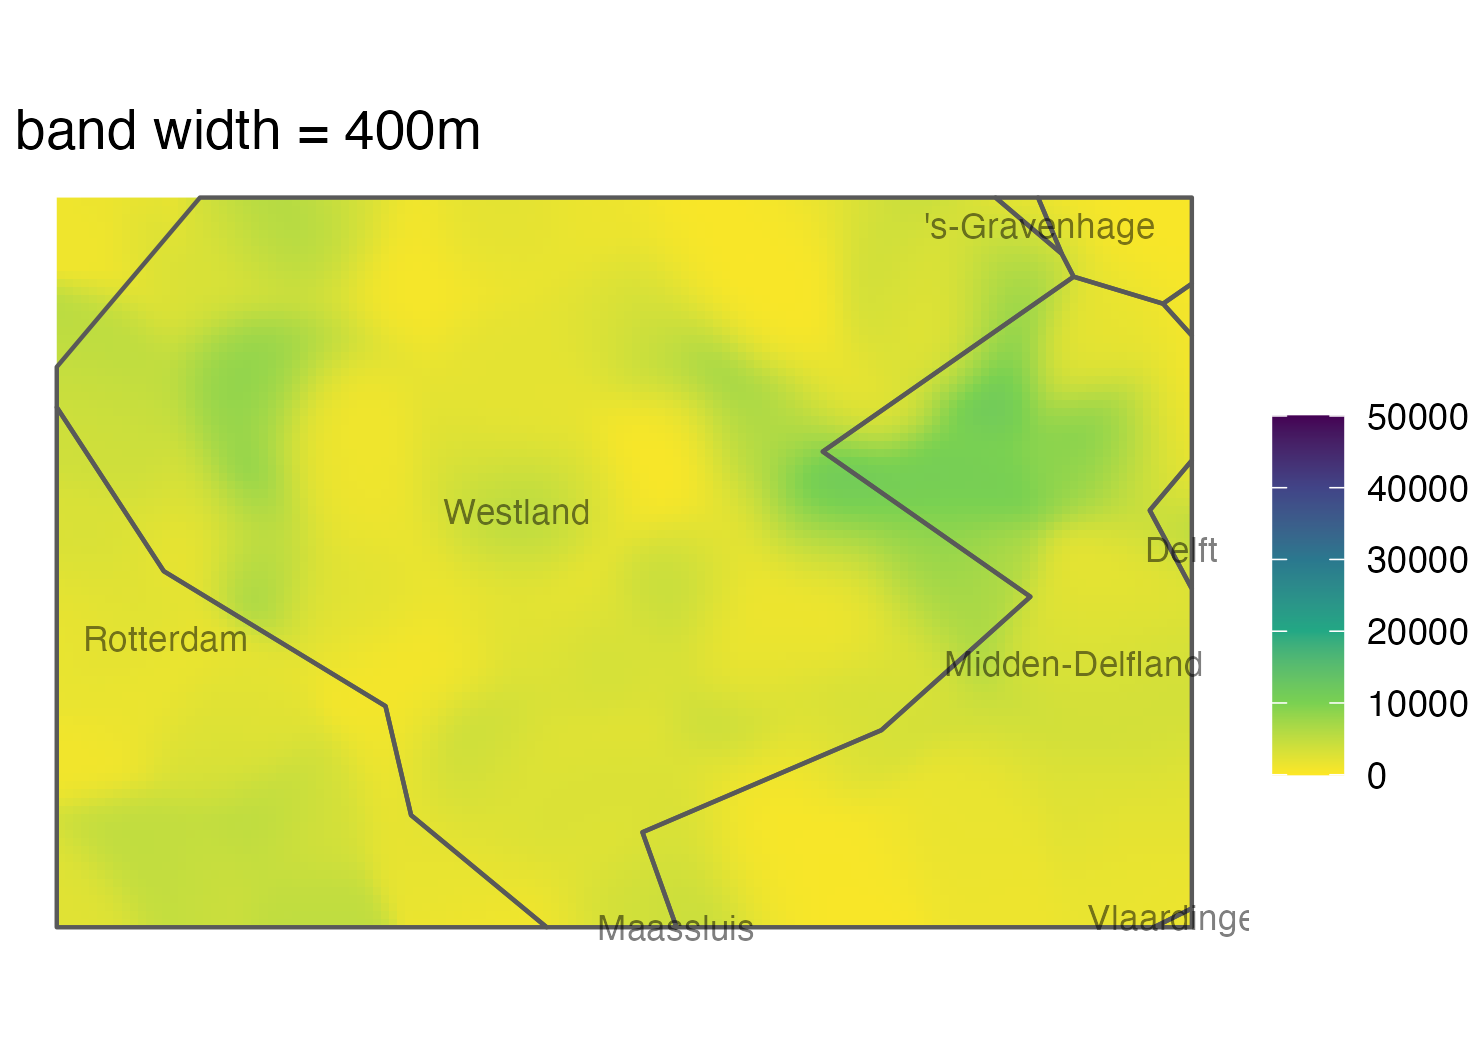
\includegraphics[width=.49\linewidth]{figures/Smoothing/fixed_smooth_400.png} 
    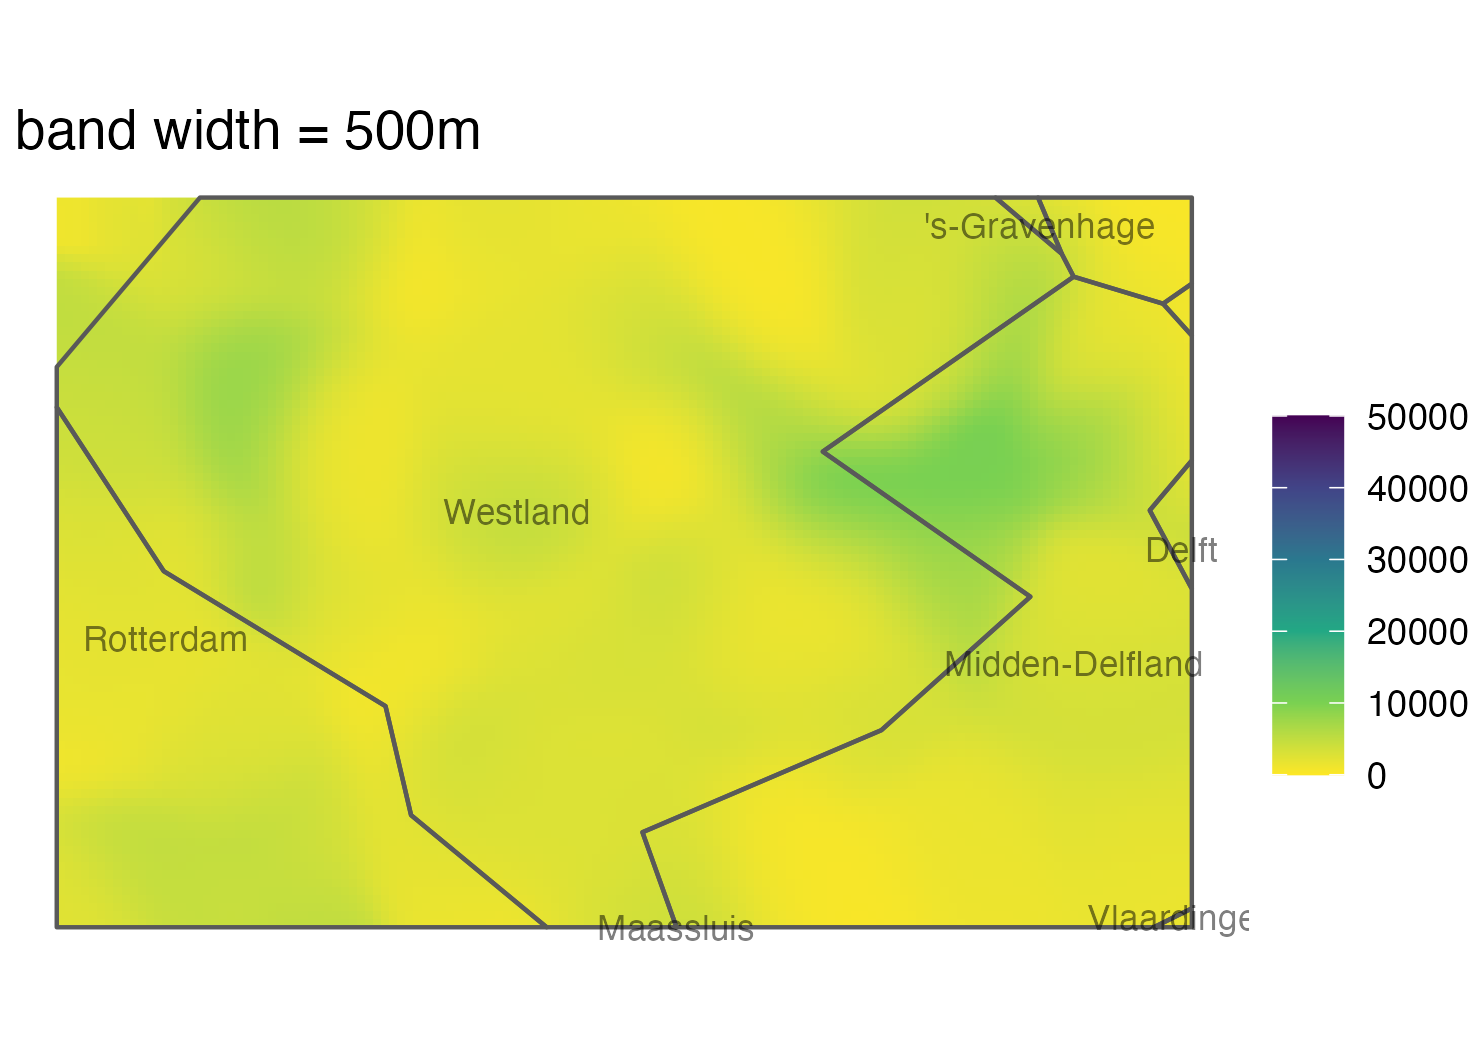
\includegraphics[width=.49\linewidth]{figures/Smoothing/fixed_smooth_500.png} 
    \caption{Spatial smoothing with increasing band width (0-500m).}
    \label{fig:sm_bandwidth}
\end{figure}

\subsection{Discussion}

An attractive feature of the kernel smoothing is that it both reveals the spatial patterns and better protects the individual observations. 
Two parameters are important for the disclosure control: band width and resolution of the data. Coarsening the grid is a simple solution for reducing disclosure risk, but also decreases utility as it quickly results in a blocky picture. 

The smoothing procedure in this section uses a fixed band width for the region. Since the spatial distribution of geographical phenomena in general is very skewed (e.g. the population densities of urban and rural regions are
very different), a variable or adaptive band width method might be interesting.

\subsubsection{Tools and Software}

Spatial smoothing for variable and population counts can be implemented with several R packages 
including \texttt{spatstat} \citep{spatstat_2005}, \texttt{btb} \citep{btb_2022} and \texttt{sdcSpatial} \citep{sdcSpatial_2022} which all assume georeferenced data. 

Spatial smoothing for population counts can also be accomplished using R packages \texttt{KernSmooth} \citep{kernsmooth_2024} and \texttt{MASS} \citep{mass_2002}.

The spatial smoothing method can be implemented using the R package \texttt{sdcSpatial} \citep{sdcSpatial_2022}. It includes options to specify the risk norms for the $p\%$ rule and the $(n,k)$ rules as well as the band width applied.
The package furthermore allows to assess the number of cells at risk and their removal.

\subsection{Summary}

Apply Spatial Smoothing to protect spatial density has the following advantages and disadvantages:

\noindent\emph{Advantages:}
\begin{itemize}
    \item Uses high density areas to protect nearby low density areas.
    \item Results in a smooth spatial density, which often aligns with publishing the data as a density map.
\end{itemize}

\noindent\emph{Disadvantages:}
\begin{itemize}
    \item Scores lower on utility measures compared to other methods.
\end{itemize}
    
\newpage